%!TEX encoding = IsoLatin

%% Document is article 
\documentclass[a4paper]{report}

%% ----------------------------------------------------- PACKAGES ----------------------------------------------------- %%
\usepackage{coolReport}
\usepackage{algorithm2e}
\graphicspath{{./Images/}}
\cRTitle{Semester project report}

%% ---------------------------------------------------------TITLE --------------------------------------------------------- %%

%% ---------------------------------------------------- DOCUMENT ---------------------------------------------------- %%
\begin{document}
	%!TEX encoding = IsoLatin


%% ------------------------------------------------------- PATHS ------------------------------------------------------- %%

%% --------------------------------------------------- PAGE STYLE --------------------------------------------------- %%

%% ---------------------------------------------------- DOCUMENT ---------------------------------------------------- %%


\begin{titlepage}
        	{\sffamily
	\large
        		\noindent \'ECOLE POLYTECHNIQUE FEDERALE DE LAUSANNE \\
        		MT SECTION\\
        		FAURY Louis \\
        	}
	
	\vfill 
        \begin{center}
   		{\sffamily\Huge
         		\textbf{SEMESTER PROJECT REPORT} \\
			\vspace{0.3cm}
			\Large
			\textbf{LASA}
		}
		\vspace{1cm}
	
        		
\includegraphics[width=0.8\textwidth]{epfl_logo.png}
        
        		\vspace{1cm}
         
         	\sffamily\huge\textbf{ 	
\titlebox{0.95}{\sffamily\huge\textbf{Learning from suboptimal demonstrations: the role of compliance in the exploration-exploitation trade-off}} }
        \end{center}
        
	\vspace{2cm}
         \centering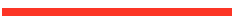
\includegraphics[width=0.1\textwidth]{sepLine}
         \vspace{0.2cm}

	\large
        \begin{center}
		\begin{tabular}{rl}
    			\textbf{Laboratory} & Learning Algorithms and Systems Laboratory (LASA)\\
			\textbf{Professor} & Prof. Aude Billard \\
    			\textbf{Supervisors} & Mahdi Khoramshahi and Andrew Sutcliffe\\
			\textbf{Semester} & Spring 2017\\
		\end{tabular}
	\end{center}
	\vspace{0.05cm}
         \centering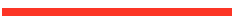
\includegraphics[width=0.1\textwidth]{sepLine}
         \vspace{0.6cm}
         \vfill
\end{titlepage}

	
	\tableofcontents

	
	\chapter{Introduction}
	{
		\section{Motivations}
		{
			\paragraph{} When it comes for real world manipulation tasks, common machine learning algorithms are sometimes unable to come up with feasible solutions, or at least fail to do so in an acceptable computational time. A natural way to accelerate the learning process is to provide a learning algorithm with prior belief on its environment, as well as recommandations with respect to the task it is trying to learn. 
			
			\paragraph{} Such prior belief is often provided thanks to demonstrations, performed by a human teacher. If this approach is largely covered in the literature (see \ref{subsection::lfd}), it is not really clear how to learn from a suboptimal teacher, regardless of its level of sub-optimality. We call \emph{largely} suboptimal a teacher providing demonstrations with potential danger or obvious downside for the robot. 
			
			\subsection{Motivating examples}
			\paragraph{} For instance, let's consider the example of a robotic arm learning to grasp an object : an unexperienced teacher might provide it with demonstrations that operate near the robot's workspace edges (which is often undesirable in robotics). Even if the robotic arm should not trust this demonstration if it wants to learn an optimal solution, simply discarding it is unwise, since it contains many important informations relative to the task (pose of the object, joint coordination, .. ). We must therefore find a way to handle the demonstration to infer those parameters without falling in its suboptimal reproduction. 
			
			\paragraph{} Before going any further, let us rephrase the previous problem slightly differently.  Indeed, we can draw a parallel between the latest example and the one of a children learning to dance (or any other technical skill). Because the child's dance teacher doesn't have the same physical abilities than the child, he might give the child a suboptimal way (with respect to the child's physical abilities) of performing dance moves. In a ideal learning process, the child would use the prior information given by the teacher, and use it to practice its skill. He will soon be aware of its own abilities, and can then start learning by itself, exploring around what he has learnt so far. He might find that, by slightly changing how he performs some moves,  he is able to dance better than by blindly listening to the teacher. Therefore, the learning child will first be \emph{compliant} with the teacher, before trying things out by itself once it has become pretty good at performing the learned skill. 
			
			\subsection{Goal}
			\paragraph{} This semester project aims at introducing a theoretical formulation of such a compliance-based behavior, and experimentally test its performance on simple problems.
			
			\paragraph{} The underlying goal behind this objective is to get better intuition about how interactive learning between human and robots can be achieved. Indeed, we would like to be able to teach a robot from demonstration not by only by providing it a large number of trajectories that he will then use as a motion generator, but by directly interacting with him. By showing a robotic arm, at different times of its learning procedure, concrete examples on how to avoid its closest obstacle and grab a given object, seems like a more natural way of teaching the robot a task, while still enabling him to correct some small sub-optimality we could have introduced to it. 
			
			\paragraph{} This approach also allows use to tackle a somehow different problem, related to transfer learning. Indeed, the teacher might not be a human but another learner, only better trained than the current learner. In such a case, we would like our learner to quickly find if it can trust its mentor, and if not where it should focus its computations to overcome its mentor's sub-optimality. Such questions will therefore be tackled in this report. 
		}
		\section{Background}
		{
			\paragraph{} We hereinafter introduce some notions from the Learning from Demonstration (LfD) framework, as well as some transfer learning metrics that will show useful later on. 
			\subsection{Learning from demonstration}
			{
				\label{subsection::lfd}
				\paragraph{} Learning from demonstration (LfD) is a framework where a robot can learn from interacting with a human. It particularly focus on the case where a mentor (human) provides demonstration on how to perform a task. Such an approach is also known as Programming from Demonstration (PbD) or Imitation Learning. 
				
				\paragraph{} LfD mostly lies on the principle that the learning robot can be taught new tasks by end-users, without having to be programmed again. We therefore are dealing with robots that are able to generalize from demonstration, be it only to understand what is the task that they must learn. They are many underlying problematics and opened questions on the subject, detailed in \cite{Billard2016}.
				
				\paragraph{}Many LfD approaches are combined with reinforcement learning techniques. This is mostly related to the understanding that demonstrations can easily speed-up the reinforcement learning process by providing a finite or infinite set of good solutions. However, this assume some kind of reproducibility by the robot, as well as a similar enough context between demonstration and reproduction. \newline
				Under such assumptions, reinforcement learning techniques can use LfD to speed up their process and discover new control policies through a directed exploration of its action-state space. Indeed, demonstrations are used to guide the reinforcement learning algorithm's exploration, reducing the time and iterations needed for an agent to discover a new control policy, and eventually overcoming the teacher's  policy sub-optimalities. 
				
				\paragraph{} They are many ways of performing such a demonstration-based learning. We remind here a few of them, taken from \cite{argall2009survey}, all related to Imitation Reinforcement Learning (IRL) : 
				\begin{itemize}
					\item policy derivations techniques : directly approximate the robot's mapping from state to action by reproducing and generalizing the teacher's one. 
					\item use demonstration data to learn a model from the world's dynamic (or transition probability model) to compute the optimal policy (see \cite{price2003accelerating}). 
					\item use demonstration data and additional user intention to learn the rule that associate a set of pre and post-conditions which each action as well as a sparse transition model to plan for actions. 
				\end{itemize}
				
				\paragraph{} The framework we described hereinbefore can easily be extended to more than one teacher. Moreover, such teachers can actually be other learning algorithms with different levels of training. Quickly, the problem drifts toward the underlying issue of performing transfer skill between agents. As this will also be tackled during this project, the next section reminds a few useful facts about the theory of transfer learning. 
			}
			\subsection{Transfer learning}
			{
				\paragraph{} Transfer learning deals with speeding a learning process thanks to another learning experience - for instance training an agent based on the previous training on another agent, performing a similar task. The literature of transfer learning in reinforcement learning is pretty large, and for a full description of the different problematics (homogeneous / inhomogeneous sets of actions, multi task learning, ..) we'll refer to \cite{taylor2009transfer}. 
				
				\paragraph{} As we said before, one of our goal is to assess our method as a transfer learning one, and up to a point, consider our teacher to be a trained (fully or not) agent, before considering many different agents as potential mentors. We would consider a really simple case of transfer learning, where all agents display the same state-action state, with the same abilities and constraints. 
				
				\paragraph{} Hence, we remind here some metrics to evaluate transfer learning methods that we would have to use to compare our different approaches : 
				\begin{itemize}
					\item \emph{Jump start} : the initial performance of an agent can be improved by transfer. 
					\item \emph{Asymptotic performance} : how close is the asymptotic learned policy from the optimal policy ? 
					\item \emph{Total or averaged reward} : averaged reward may be improved by transfer 
					\item \emph{Transfer ratio} : Ratio of total reward accumulated by the transfer learner and the total of reward accumulated by a non-transfer learner. 
					\item \emph{Time to threshold} : the time required by a transfer learning to reach a pre-specified level of skills in achieving its task. 
				\end{itemize}
				
				\paragraph{} All those metrics actually compared different aspects of how well a RL algorithm learns. Comparing two reinforcement learning methods is actually still an open question, and hence we'll need to address several of those metrics to decide on the wellness of our derived TL methods. 
			}
		}
		\section{Outline}
		{
			
			\paragraph{} To grasp ideas and intuitions about a compliant-based imitation learning method, we are going to start with a fairly simple environment and an explicit task. We hope that a simple enough state space will allow us to better understand how compliance in learning by demonstration should be tackled with a reinforcement learning formulation.  We also hope we would be able to generalize to more complex situations once the understanding on a simple but generic model is mastered. 
			
			\paragraph{} Hence, after defining a simple two dimensional grid-world state space with a simple action set, we will quickly study how well the different classical reinforcement learning policy search algorithms performs on such a space. We will then introduce new exploration policies, based on the confidence the learner has in its teacher and compare their efficiency with the latter algorithms. We will also focus on the relation between the learner and the prior information that its mentor's recommandations represent. Especially, we will study how well a learner can overcome its mentor own sub-optimality, focusing on largely suboptimal mentors. 
		}
	}
	\newpage
	
	\chapter{Reinforcement Learning}
	{
		\paragraph{} The reinforcement learning approach being an essential aspect of this project, this chapter is intended to remind the foundations of the reinforcement learning theory and its practical implementations. 
		\section{Formulation}
		{
			\subsection{Definitions}
			{
				\paragraph{} Reinforcement learning is a framework in which an \emph{agent} (or a \emph{learner}) learns its actions from interaction with its environment. The environment generates scalar values called \emph{rewards}, that the agent is seeking to maximize over time. 
			
				\paragraph{} Let $\mathcal{S}$ denote the state space in which our agent evolves (the localization of a robot on a grid for instance), and $\forall{s}\in\mathcal{S}$ we will define the action state $\mathcal{A}(s)$, describing all possible action that can be taken by the agent at state $s$. When taking an action from a state $s_t$, the agent finds itself in a new state $s_{t+1}$ where it receives a reward $r_{t+1}\in\mathbb{R}$. The action taken is sampled over a probability distribution from the joint space of state and action : 
				\begin{equation}
					\begin{aligned}
						\pi \, : \, \mathcal{S}\times\mathcal{A}(s) \, &\to [0,1]\\
							 (s,a) \, &\to \,  \pi(s,a)
					\end{aligned}
				\end{equation}	
				where $\pi(s,a)$ is the probability of picking action $a$ in state $s$. Such a distribution is called the agent's \emph{policy}. The key goal of reinforcement learning is teaching an agent on how to change its policy to maximize its reward on the long run. 
				
				\paragraph{} The agent indeed seeks to maximize the \emph{expected return} $R_t$ mapping the reward sequence into $\mathbb{R}$. A commonly used expression for this value employs a \emph{discount factor} $\gamma \in [0,1]$, allowing to make the agent's more sensible to rewards it will get in a close future : 
				\begin{equation}
					R_t = \sum_{i=0}^T \gamma^i r_{t+1+i}
				\end{equation}
				This also allows to adapt this formulation to continuous tasks, where there are no terminal states and the task goes on indefinitely (there are no \emph{episodes} in the learning). 
				
				%% TODO : quote Sutton's book 
			}
			\subsection{Markov decision process}
			{
				\paragraph{} To make the problem tractable, we ask for the state signal to comply with Markov's property, hence to be \emph{memory-less}. For instance, we want to be able to write that, in a stochastic environment, $\forall s'\in\mathcal{S}$ : 
				\begin{equation}
					\mathbb{P}\left( s_{t+1}=s' \, \vert \, a_t, s_t, \hdots, a_1,s_1\right) = \mathbb{P}\left( s_{t+1}=s' \, \vert \, s_t, a_t\right)
				\end{equation}
				
				\paragraph{} Hence, every reinforcement learning problem can be represented by a \emph{Markov Decision Process}, that consists in a 5-tuple $\left(\mathcal{S}, \mathcal{A}, \mathcal{P}_{\cdot}(\cdot,\cdot), \mathcal{R}_{\cdot}(\cdot), \gamma \right)$ where : 
				\begin{itemize}[label=$\triangleright$]
					\item $\mathcal{S}$ is the agent's state space
					\item $\mathcal{A}$ is the agent's action space
					\item $\forall s,s'\in\mathcal{S}, \, \forall a\in\mathcal{A}(s)$,  $\mathcal{P}_a(s,s') = \mathbb{P}(s_{t+1}=s'\, \vert \, s_t = s, a_t = a)$ is the probability that action $a$ in state $s$ will lead the agent to transitioning to state $s'$.
					\item $\forall s,s'\in\mathcal{S}, \, \forall a\in\mathcal{A}(s)$,  $\mathcal{R}_a(s,s')$ is the immediate reward perceived by the agent when transitioning from state $s$ to $s'$ when taking action $a$. 
					\item $\gamma$ is the discount factor. 
				\end{itemize}
				
				\paragraph{} A \emph{finite Markov decision process} designates a MDP for which both the action and state space are finite. 
			}
			\subsection{State and action value function}
			{
				\paragraph{} Most of the reinforcement learning algorithms are based on evaluation value function. A value function is a function mapping the state space in $\mathbb{R}$, estimating how good (in terms of expected future reward) it is for the agent to be in a given space. More precisely, a value function $V^\pi(\cdot)$ evaluates the expected return of a state when following the policy $\pi$. $V^\pi(\cdot)$ is called the \textbf{state-value function}. 
				\begin{equation}
					\forall{s}\in\mathcal{S}, \quad V^\pi(s) = \E[\pi]{R_t \, \vert \, s_t = s}
				\end{equation}
				The \textbf{action-value function} evaluates the value of taking a given action, and then following the policy $\pi$ : 
				\begin{equation}
					\forall{s,a}\in\mathcal{S}\times\mathcal{A}(s), \quad Q^\pi(s,a) = \E[\pi]{ R_t \, \vert \, s_t=s, \, a_t=a}
				\end{equation}
				
				\paragraph{} Both those functions satisfy particular recursive relationships known as the \emph{Bellman equations}. It is shown that (see TODO quote Sutton) we have the following results : 
				\vspace{10pt}
				
				\coolbox{white}{\textcolor{black}{Bellman equations for Markov Decision Process}}
				{
					\begin{itemize}[label=$\triangleright$]
						\item Bellman equation for the state-value function : $\forall s \in\mathcal{S}$ 
						\begin{equation}
							V^\pi(s) = \sum_{a\in\mathcal{A}}\pi(s,a)\sum_{s'} \mathcal{P}_a(s,s')\left[\mathcal{R}_a(s,s') + \gamma V^\pi(s')\right]
						\end{equation}
						\item Bellman equation for the action value function : $\forall{s,a}\in\mathcal{S}\times\mathcal{A}(s)$ : 
						\begin{equation}
							Q^\pi(s,a) = \sum_{s'}\mathcal{P}_a(s,s')\left[ \mathcal{R}_a(s,s') + \gamma V^\pi(s')\right]
						\end{equation}
					\end{itemize}
				}
			}
			\subsection{Optimal policies}
			{
				\paragraph{} The value functions define a partial ordering in the policy space. A policy $\pi$ is therefore said to be better than $\pi'$ (or $\pi\geq \pi'$) if $\forall{s}\in\mathcal{S}$, $V^\pi(s) \geq V^\pi(s')$. We are looking for $\pi^*$ so that : 
				\begin{equation}
					\forall\pi, \quad \pi^* \geq \pi 
				\end{equation}
				
				TODO quote showed that for finite MDPs, there is always at least one policy that is better our equal to all others, and therefore is called the \emph{optimal policy} $\pi^*$. As shown in TODO quote, the state-value and action-value function verify the \emph{Bellman optimality equations}. 
				
				\vspace{10pt}
				
								\coolbox{white}{\textcolor{black}{Bellman optimality equations}}
				{
					\begin{itemize}[label=$\triangleright$]
						\item Bellman optimality equation for the state-value function : $\forall s \in\mathcal{S}$ 
						\begin{equation}
							V^\pi(s) = \max_{a\in\mathcal{A}(s)}\pi(s,a)\sum_{s'} \mathcal{P}_a(s,s')\left[\mathcal{R}_a(s,s') + \gamma V^\pi(s')\right]
						\end{equation}
						\item Bellman optimality equation for the action value function : $\forall{s,a}\in\mathcal{S}\times\mathcal{A}(s)$ : 
						\begin{equation}
							Q^\pi(s,a) = \sum_{s'}\mathcal{P}_a(s,s')\left[ \mathcal{R}_a(s,s') + \max_{a\in\mathcal{A}(s')} Q(s',a') \right]
						\end{equation}
					\end{itemize}
				}
				
				\paragraph{} Those relations are essential in understanding the solving algorithms that will be presented later. 
			}
		}


			\paragraph{} There exists several ways of solving (i.e computing the optimal policy) of a Markov Decision Process, that can generically be separated in two categories : \emph{model-based} and \emph{model-free} methods. 
		\section{Dynamic Programing}
		{
			\paragraph{} Dynamic programing is a mathematically well-developed theory. It requires the complete and accurate model of the environment, making it a model-based method. 
			
			\paragraph{} Dynamic programing methods aims at computing the optimal value function at every state of state space. This could, of course, be done by solving the $\vert \mathcal{S} \vert $ equations of $\vert \mathcal{S} \vert $ unknowns that are the Bellman equations for a given policy, and then evolve that policy toward a better one, based on the current value function. Of course, this approach is computationally intractable for large state space and therefore needs to be adapted, but gives a first approach of the idea behind dynamic programing. 
				
			\subsection{Generalized policy iteration}
			{
				\paragraph{} The generalized policy iteration methods rely on alternating two processes, known as \textcolor{red}{policy evaluation} and \textcolor{red}{policy improvement}. 
				\begin{itemize}[label=$\triangleright$]
					\item Policy evaluation deals with estimating the value function of a given policy $\pi$, without directly solving the full system given by Bellman equations. The idea is actually pretty simple : use Bellman's equation as an update rule, using that the value function is a fixed point for this update rule. The algorithm, after setting the tabled value function to an initial value, iterate by performing what is called \emph{full Bellman backups} : 
					\begin{equation}
						\forall{s}\in\mathcal{S}, \quad V_{k+1}^\pi(s) = \sum_{a\in\mathcal{S}} \pi(s,a)\sum_{s'}\mathcal{P}_a(s,s') \left[\mathcal{R}_a(s,s')+V_k^\pi(s')\right]
					\end{equation}
					This algorithm converges under the same assumptions that guarantee the existence of the value function, and has the generic name of \emph{iterative policy evaluation}. They are many refining for speeding up that process (reduced backups, prioritized sweeping) that we won't address here. 
				\item Policy evaluation is a process that from a given policy value function, returns a better or equal policy compared to the latter. The simplest way to do that is for every state $s\in\mathcal{S}$, consider every action-value functions : 
				\begin{equation}
					Q(s,a) = \sum_{s'}\mathcal{P}_a(s,s')\left[\mathcal{R}_a(s,s') + \gamma V\pi(s')\right], \quad a\in\mathcal{A}(s)
				\end{equation}
				and to build $\pi'$ to be \emph{greedy} with respect to those actions-values : 
				\begin{equation}
					\pi'(s) = \argmax{a\in\mathcal{A}(s)}{Q(s,a)}
				\end{equation}
					The policy improvement theorems then ensures that $\pi'\geq \pi$. 
				\end{itemize}
				
				\paragraph{} Hence, generalized policy improvement are a set of methods that iteratively combine those two sub-methods to compute the optimal policy for a given MDP. Of course, one does not have to perform all sweeps of value evaluation before improving the policy to converge toward an optima (indeed, many times our sweeps won't have any affect on the greedy policy). They are many ways to combine the two (prioritized sweeping, asynchronous dynamic programing), but the most used and one of the most quickest way to converge is to use the value iteration algorithm. 
			}	
			\subsection{The value iteration algorithm}
			{
				\paragraph{} The value iteration algorithm takes the limit of the behavior we just described, and stops the value evaluation procedure after only \emph{one state space sweep}. It therefore performs a simple backup procedure : 
					\begin{equation}
						\forall{s}\in\mathcal{S}, \quad V_{k+1}  = \max_{a\in\mathcal{A}}  \sum_{s'}\mathcal{P}_a(s,s')\left[\mathcal{R}_a(s,s') + \gamma V_k^\pi(s')\right]
					\end{equation}
					For any arbitrary $V_0$, it is shown that $V_k\to V^*$ as $k\to\infty$, under the same hypothesis that ensure the existence of the optimal value function $V^*$. As one can notice, it actually implements the \emph{Bellman optimality conditions} as an update rule !
				}
			}
		
		
		\section{Temporal differences methods}
		{
			\paragraph{} Temporal difference methods can be seen as a combination of dynamic programing and another kind of learning called Monte Carlo methods, where the expected return are approximated via sampling. Like dynamic programming, TD methods are said to bootstrap (meaning that they build their estimators through already estimated values), but are \emph{model-free} methods and learn from experience. 
			
			\paragraph{} The justification, proof of convergences and literature and those models is pretty wide, hence we will not cover them in this report. However, full description of those methods can be found in TODO quote. 
			
			\subsection{On-policy method : SARSA}
			{
				\paragraph{} The SARSA algorithm is an \emph{on-policy} control method, meaning that the algorithm updates the value function and improves the current policy it is following. At state $s_t$, it chooses an action $a_t$ from its policy and follows it. After observing the reward $r_{t+1}$ and the next state $s_{t+1}$, it again chooses an action $a_{t+1}$ using a soft policy and performs a one-step backup : 
				\begin{equation}
					Q(s_t,a_t) \leftarrow Q(s_t,a_t) + \alpha\left[r_{t+1} + \gamma Q(s_{t+1},a_{t+1}) - Q(s_t,a_t)\right]
				\end{equation}
				It therefore relies on a 5-tuple $(s_t,a_t,r_{t+1},s_{t+1},a_{t+1})$ to perform the udpate, giving it the State Action Reward State Action (SARSA) name. 
				\vspace{10pt}
				
				\coolbox{white}{\textcolor{blue}{The General Sarsa Algorithm}}
					{
						\begin{algorithm}[H]
	 					\SetAlgoLined
						\LinesNumbered
						\emph{\textsf{1. Initialize}} $Q(s,a)$ arbitrarily $\forall (s,a)\in\mathcal{S}\times\mathcal{A}(s)$ \\
						\BlankLine
						\BlankLine
						\emph{\textsf{2. Repeat}} for each episode : \\
						\Indp \Indp 
							Initialize $s$ \\
							Choose $a\in\mathcal{A}(s)$ using a soft policy derived from $Q$ (typically $\varepsilon$-greedy) \\
							Repeat for each step of the current episode :   \\
							\Indp \Indp 
								Take $a$, observe $r,s'$ \\
								Choose $a'$ from $s'$ using policy derived from $Q$ 
								$ Q(s,a) \longleftarrow Q(s,a) + \alpha\big[ r + \gamma Q(s',a') - Q(s,a) \big]$ \\
								$a\leftarrow a'$, $s\leftarrow s' $ \\
								
							\Indm \Indm 
						until $s\in\mathcal{S}^+$.
						\Indm \Indm 
						\end{algorithm}
					}
					
					\paragraph{} The convergence properties of SARSA depend on the nature of the policy's dependency on Q. Indeed, SARSA converges with probability 1 to the optimal policy as long as all the sate and actions pairs are visited an infinite number of time, and the policy converges in the limit to the greedy policy. This is done, for instance, by turning the temperate of a softmax based policy to 0, or by having $\eps\to 0$ for a $\eps$-greedy policy. For SARSA to converge, we also as the learning rate to comply with the stochastic approximation conditions : 
					\begin{equation}
						\sum_k \alpha_k(a) = +\infty \quad { and } \quad \sum_k \alpha_k(a)^2 < +\infty
					\end{equation}
					where $\alpha_k(a)$ is the learning rate for the k\textsuperscript{th} visit of the pair $(s,a)$. 
					
			}
			\subsection{Off-policy method : Q-learning}
			{
				\paragraph{} The Q-learning algorithm is an off-policy method who learns to directly approximate $Q^*$, independently of the policy being followed. Its update rule is given by :
				\begin{equation}
					Q(s_t,a_t) \leftarrow Q(s_t,a_t) + \alpha \left[ r_{t+1} + \gamma \max_{a\in\mathcal{A}(s_{t+1})} Q(s_{t+1},a) - Q(s_t,a_t)\right]
				\end{equation}
				The actual policy being followed still has an effect in that it determines which state-actions pairs are visited and updated. However all that is required for convergence it that all pairs continue to be updated. 
				\vspace{10pt}
				
				\coolbox{white}{\textcolor{blue}{Q-Learning Algorithm}}
					{
						\begin{algorithm}[H]
	 					\SetAlgoLined
						\LinesNumbered
						\emph{\textsf{1. Initialize}} $Q(s,a)$ arbitrarily $\forall (s,a)\in\mathcal{S}\times\mathcal{A}(s)$ \\
						\BlankLine
						\BlankLine
						\emph{\textsf{2. Repeat}} for each episode : \\
						\Indp \Indp 
							Initialize $s$ \\
							Repeat for each step of the current episode :   \\
							\Indp \Indp 
								Choose $a\in\mathcal{A}(s)$ using arbitrary policy \\
								Take $a$, observe $r,s'$ \\
								$ Q(s,a) \longleftarrow Q(s,a) + \alpha\big[ r + \gamma \max_{a'\in\mathcal{A}(s')}Q(s',a') - Q(s,a) \big]$ \\
								$s\leftarrow s' $ \\
								
							\Indm \Indm 
						until $s\in\mathcal{S}^+$.
						\Indm \Indm 
						\end{algorithm}
					}
				
				\paragraph{} Along with this hypothesis and a slight variation in the usual stochastic approximation conditions, the learned action value function by Q-learning has been shown to converge to $Q^*$ with probability $1$. 
			}
			\subsection{Eligibility traces}
			{
				\paragraph{} In TD(0) approach (described in the latest section), we update the value function in the direction of the \emph{one-step return} : 
				\begin{equation}
					\Delta V_t(s_t)^{(1)} = \alpha \left[ r_t + \gamma V_t(s_{t+1}) - V_(s-t)\right]
				\end{equation}
				The idea behind eligibility traces is to expand that update rule in order to steer the value fonction towards the \emph{n-step return} (or at least until a terminal state is reached) :
				\begin{equation}
					\begin{aligned}
					\Delta V_t(s_t) ^{(n)} &= \alpha \left[ r_t + \gamma r_{t+1} + \hdots + \gamma^{n} V_t(s_{t+n})-V_t(s_t)\right]	\\
									&= \alpha \left[R_t^{(n)} - V_t(s_t)\right]
					\end{aligned}
				\end{equation}
				
				\paragraph{} The backups can not only be done toward any n-step return, but toward any average of such returns, as long as the corresponding weights sum-up to one. In this way, the TD($\lambda$) algorithm can be understood as a particular way of averaging $n$-steps returns. With $\lambda<1$, the resulting backup is known as the \textcolor{red}{\emph{$\lambda$-return}} : 
				\begin{equation}
					R_t^\lambda = (1-\lambda) \sum_{n=1}^\infty \lambda^{n-1}R_t^{(n)}
				\end{equation}
				where the weights are fading with $n$. When the runs are episodic, we can write this return as : 
				\begin{equation}
					R_t^\lambda = (1-\lambda)\sum_{n=1}^{T-t-1} \lambda^{n-}R_t{(n)} + \lambda_{T-t-1}R_t^{(T)}
				\end{equation}
				
				\coolbox{white}{\textcolor{blue}{Sarsa($\lambda$) algorithm}}
					{
						\begin{algorithm}[H]
						\label{sarsalambda}
	 					\SetAlgoLined
						\LinesNumbered
						\emph{\textsf{1. Initialize}} $Q(s,a)$ arbitrarily $\forall (s,a)\in\mathcal{S}\times\mathcal{A}(s)$ \\
						\BlankLine
						\BlankLine
						\emph{\textsf{2. Repeat}} (for each episode) : \\
						\Indp \Indp 
							Initialize $s,\, a$ \\
							Repeat for each step of the current episode :   \\
							\Indp \Indp 
								Take action $a$, observe $r, s'$. \\
								Choose $a'\in\mathcal{A}(s')$ using soft policy derived from $Q$\\
								$\delta \longleftarrow r + \gamma Q(s',a') - Q(s,a)$ \\
								$e(s,a) \longleftarrow e(s,a) +1 $\\
								For all $s,a$ : \\
								\Indp \Indp 
									$ Q(s,a) \longleftarrow Q(s,a) + \alpha \delta e(s,a) $ \\
									$ e(s,a) \longleftarrow \gamma \lambda e(s,a) $\\
								\Indm \Indm 
								$s\leftarrow s'$, $a\leftarrow a'$\\						
							\Indm \Indm 
						until $s\in\mathcal{S}^+$.\\
						\Indm \Indm 
						\end{algorithm}
					}


				\paragraph{} Such a formulation of eligibility traces is known as the \emph{\textcolor{red}{forward view}} of TD($\lambda$), and shows how eligibility traces build the bridge between TD(0) methods and Monte-Carlo one. It is not implementable as is since it is non-causal. There exist a more mechanistic view, equivalent to the forward view (see \cite{Sutton98a}), known as the \emph{backward-view}. It gives birth to causal version of the TD($\lambda$) method. We give as an example the pseudo-code for the SARSA($\lambda$) algorithm above. Its Q-learning equivalent can be found in \cite{Sutton98a}.   
			}
		}
	
		\section{Grid-world examples}
		{
			\paragraph{} We hereinafter describe two grid-world state spaces, on which we will apply the learning rule derived in the latest section. Such example are trivial and are displayed here just to show convergence and behavior of the different algorithms. 
			
			\paragraph{} We'll consider the two following state spaces : 
			\begin{figure}[ht!]
				\begin{minipage}{0.4\linewidth}
					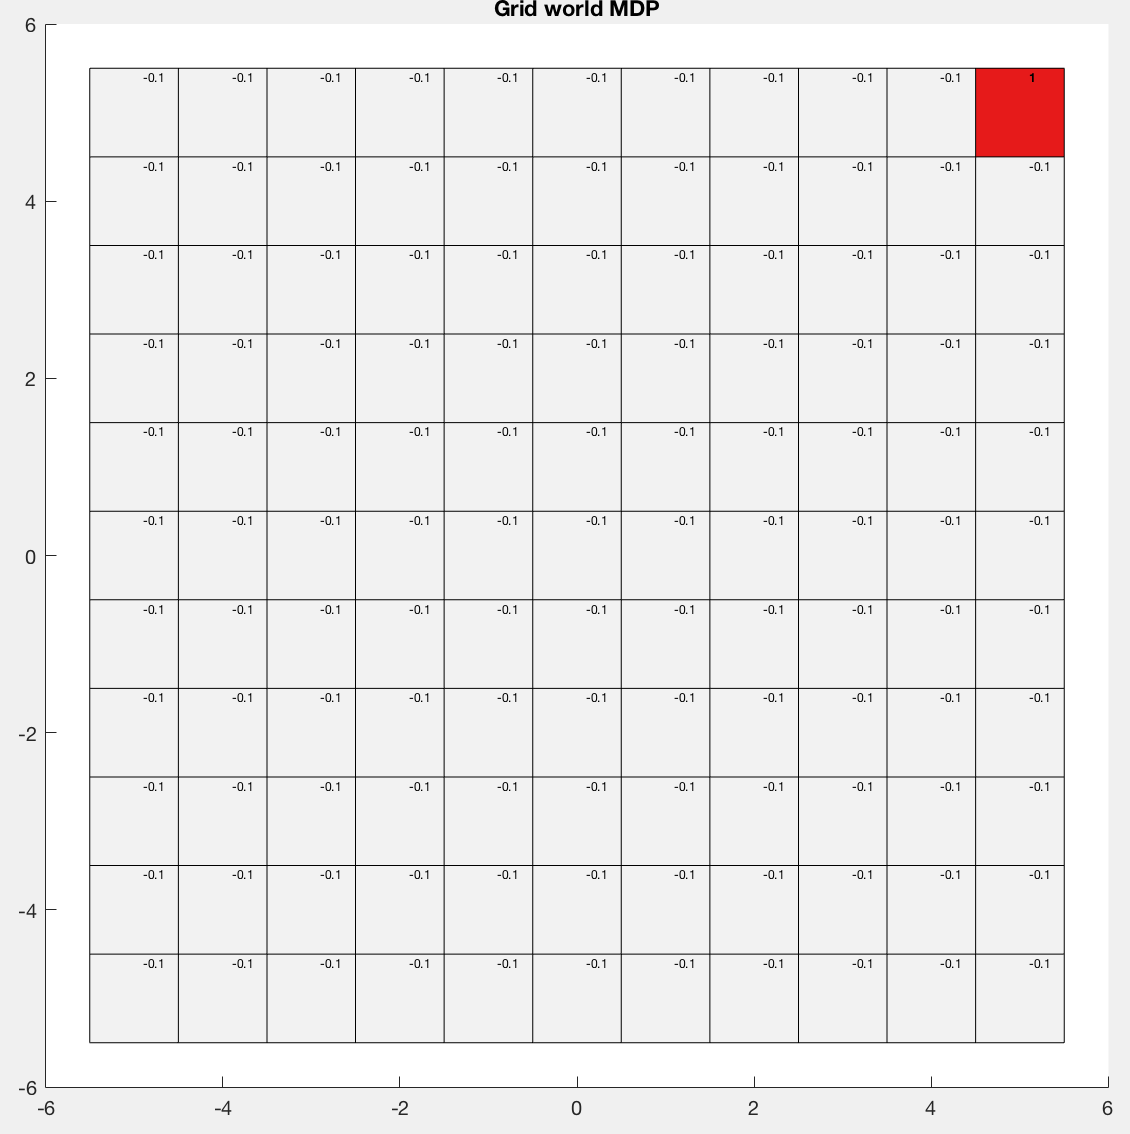
\includegraphics[width=\linewidth]{free_grid}
					\caption{The \emph{free\_grid} state space}
				\end{minipage}
				\hfill
				\begin{minipage}{0.4\linewidth}
					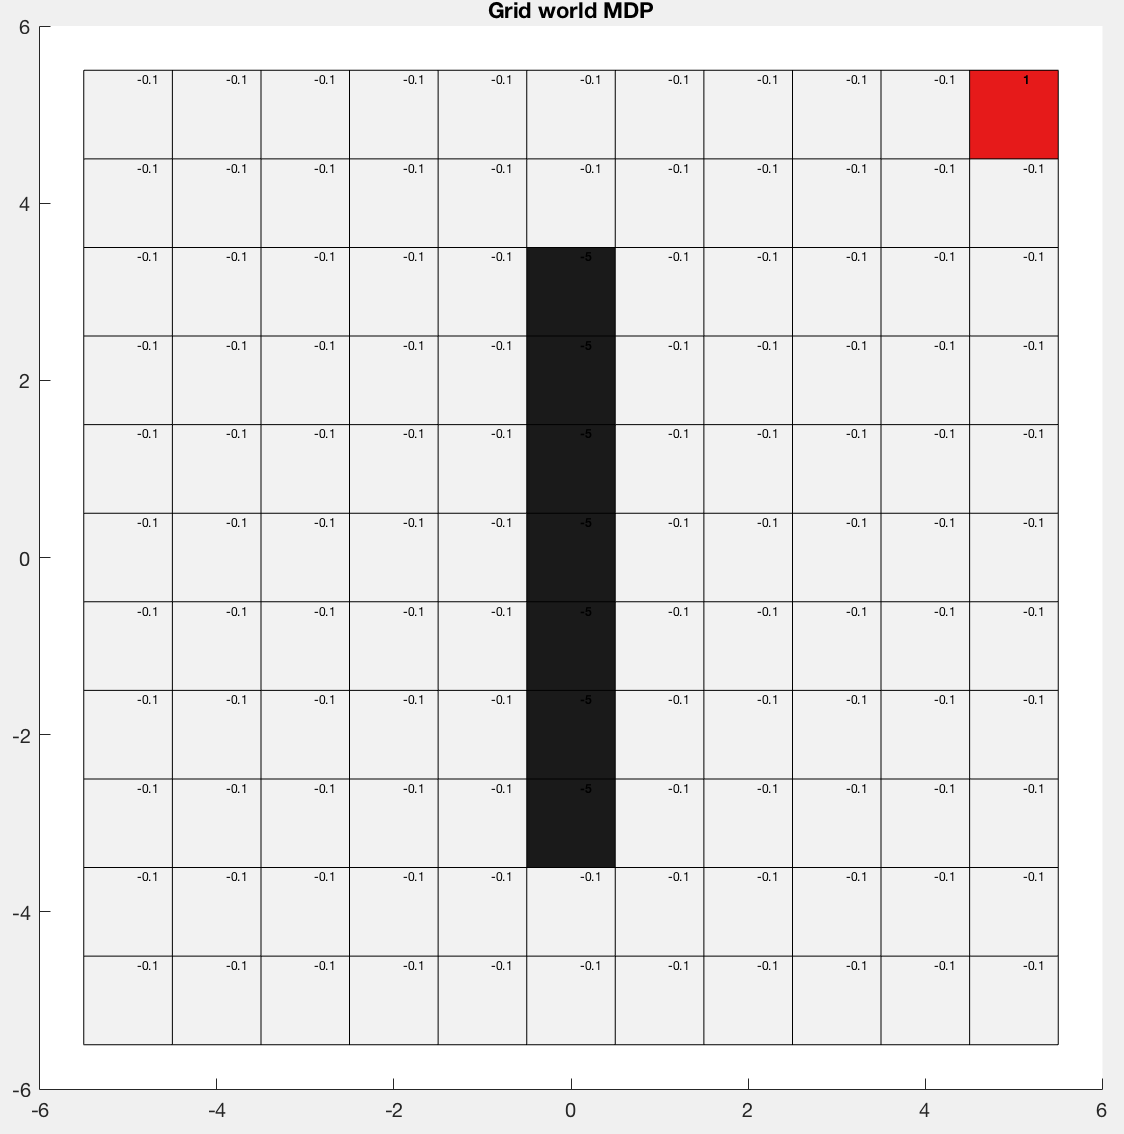
\includegraphics[width=\linewidth]{bar_grid}
					\caption{The \emph{bar\_grid} state space}
				\end{minipage}
			\end{figure}
			\subsection{Dynamic Programing solving}
			{
				\paragraph{} Let us run the DP algorithm on such grid worlds. We'll consider a stochastic environnement, with the transition probability : 
				\begin{equation}
					\mathcal{P}_{s,s'}^a = \left\{\begin{aligned} &0.9 &\text{ if }s' = a(s) \\ &0.1 &\text{ otherwise} \end{aligned}\right.
				\end{equation}
				Running the value iteration algorithm (assuming we now the environment model), we obtain the following policies and learning curves. The stopping criterion adresses the maximum absolute change brought to the value function as the sweeping goes through the state space : 
				\begin{equation}
					\text{ If } \max_{s\in\mathcal{S}} \vert V_{k+1}(s) - V_k \vert < \delta \text{ then stop}
				\end{equation}
				
				\begin{figure}[ht!]
				\begin{minipage}{0.4\linewidth}
					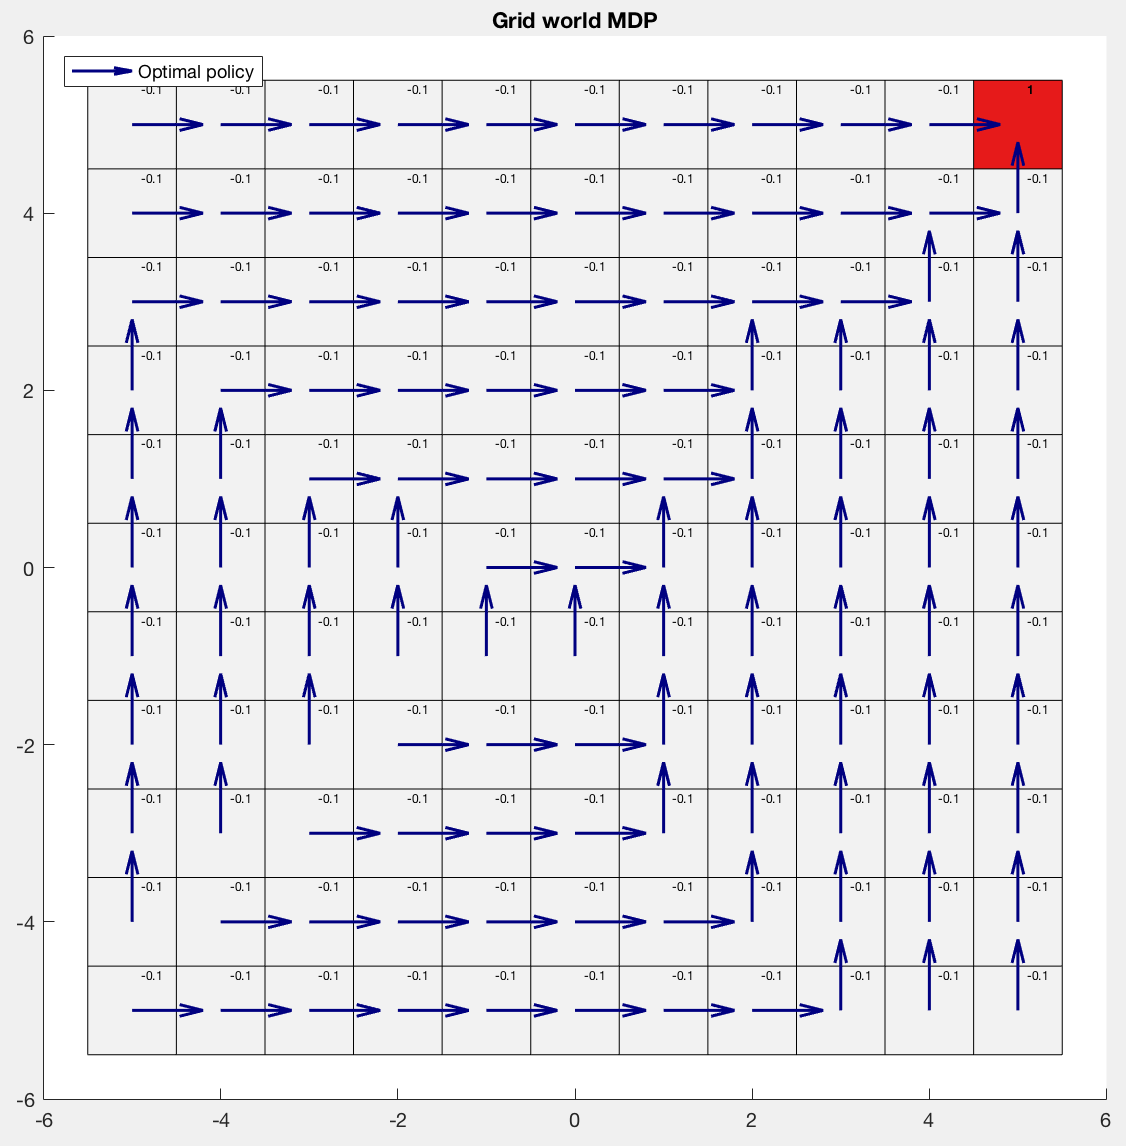
\includegraphics[width=\linewidth]{free_grid_bellman_policy}
					\caption{The \emph{free\_grid} learned optimal policy}
				\end{minipage}
				\hfill
				\begin{minipage}{0.4\linewidth}
					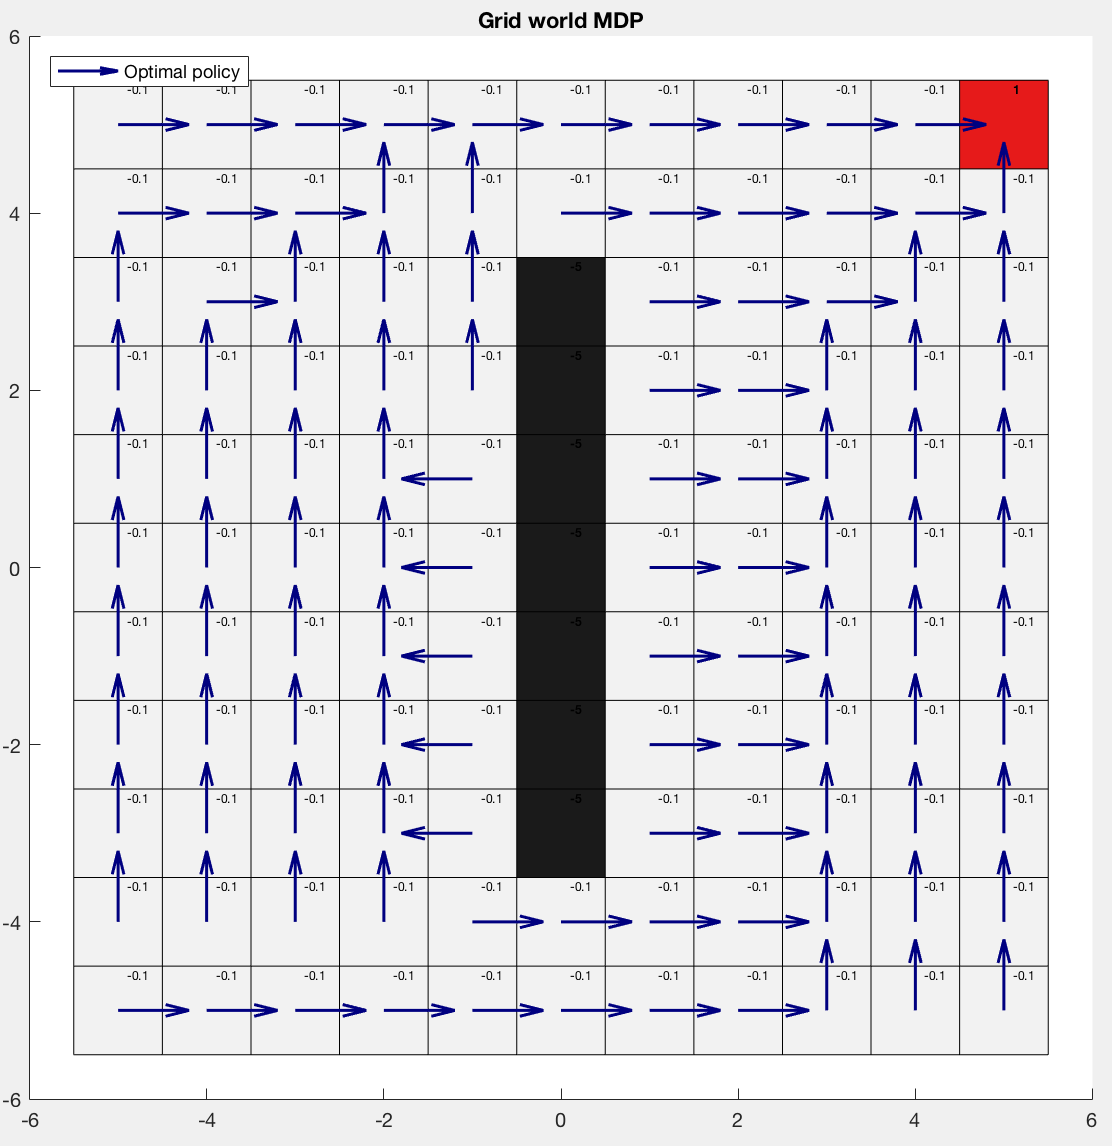
\includegraphics[width=\linewidth]{bar_grid_bellman_policy}
					\caption{The \emph{bar\_grid} learned optimal policy}
				\end{minipage}
				\end{figure}
				
				\begin{figure}[ht!]
				\begin{minipage}{0.4\linewidth}
					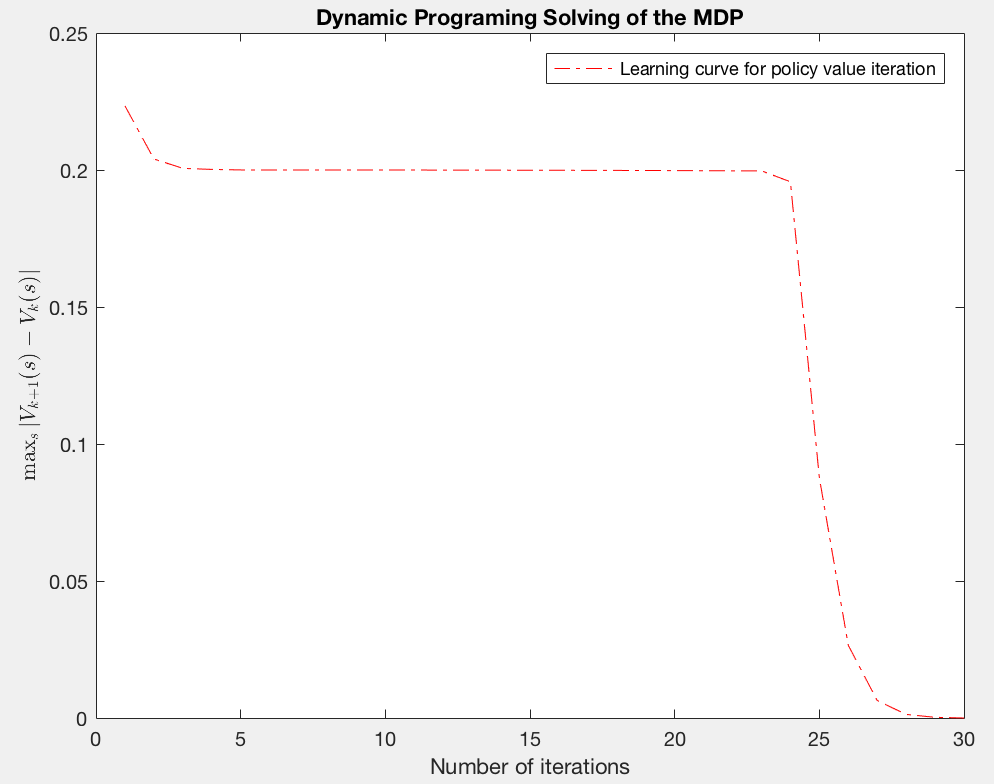
\includegraphics[width=\linewidth]{free_grid_bellman_lc}
					\caption{The \emph{free\_grid} value iteration learning curve}
				\end{minipage}
				\hfill
				\begin{minipage}{0.4\linewidth}
					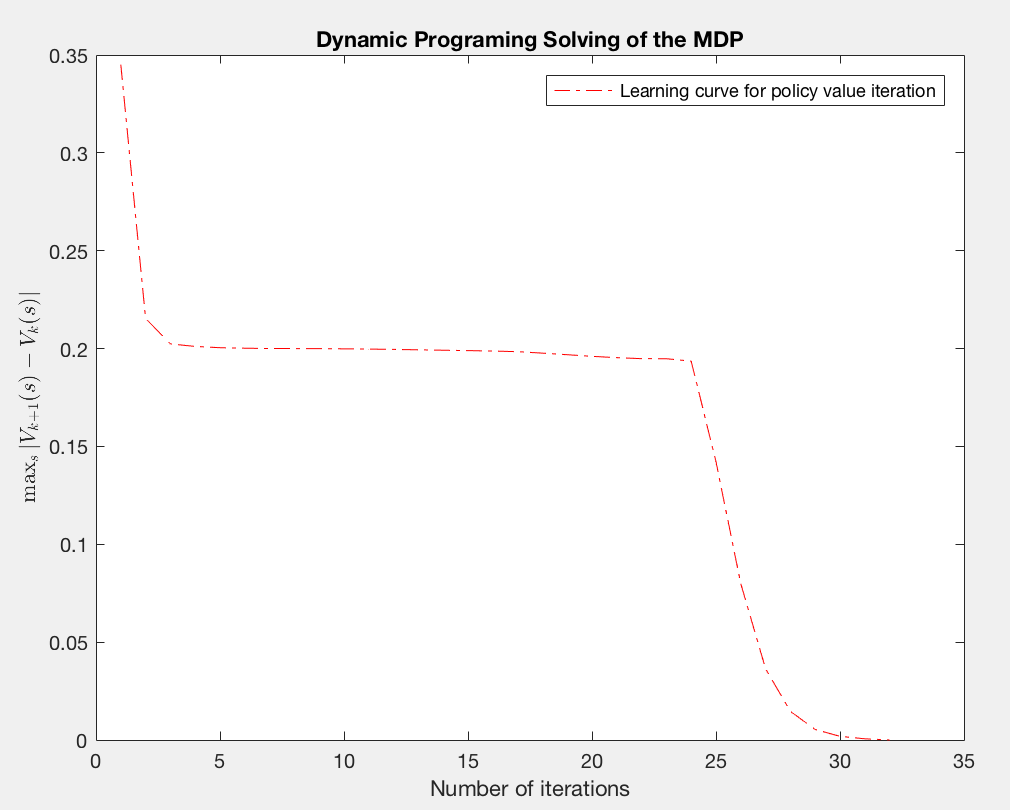
\includegraphics[width=\linewidth]{bar_grid_bellman_lc}
					\caption{The \emph{bar\_grid} value iteration learning curve}
				\end{minipage}
				\end{figure}
				
				\paragraph{} One can notice that for the \emph{bar\_grid} environment, the agent undergoes a longer trajectory than necessary, at the left of the obstacle. This is because of the stochastic nature of the environment, causing the agent to learn to takes its distance with the obstacle in order not to accidentally hit it (and then receive a very negative reward). 
				
				\paragraph{} The learned policy are indeed optimal. The next algorithms (SARSA and Q-learning) will try to reproduce them without a model for the environment. 
			}
			\subsection{SARSA solving}
			{
				\paragraph{} We display here the learning curves for the \emph{free\_grid} state space using SARSA. The algorithm manages to learn the optimal policy and the right action-value functions. We use \emph{optimistic initialization} to encourage exploration, and Gibbs sampling for following a soft-policy : $\forall (s,a) \in\mathcal{S}\times \mathcal{A}(s)$ 
				\begin{equation}
					\pi(s,a) = \displaystyle \frac{ e^{Q(s,a)/\tau}}{\sum_{a'\in\mathcal{A}(s)}e^{Q(s,a')/\tau}}
				\end{equation}
				We'll tune the distribution's temperature $\tau$ to zero, in order to converge toward the greedy policy w.r.t the learned action-value function. 
				
				\paragraph{} Following this strategy and tuning our learning rate to comply with the stochastic approximation conditions, we obtain the following learning curves. Again, our stopping criterion addresses the \emph{maximum change in the acton-value function over all the trajectories of a mini-batch}. 
				\begin{figure}[ht!]
					\begin{minipage}{0.4\linewidth}
						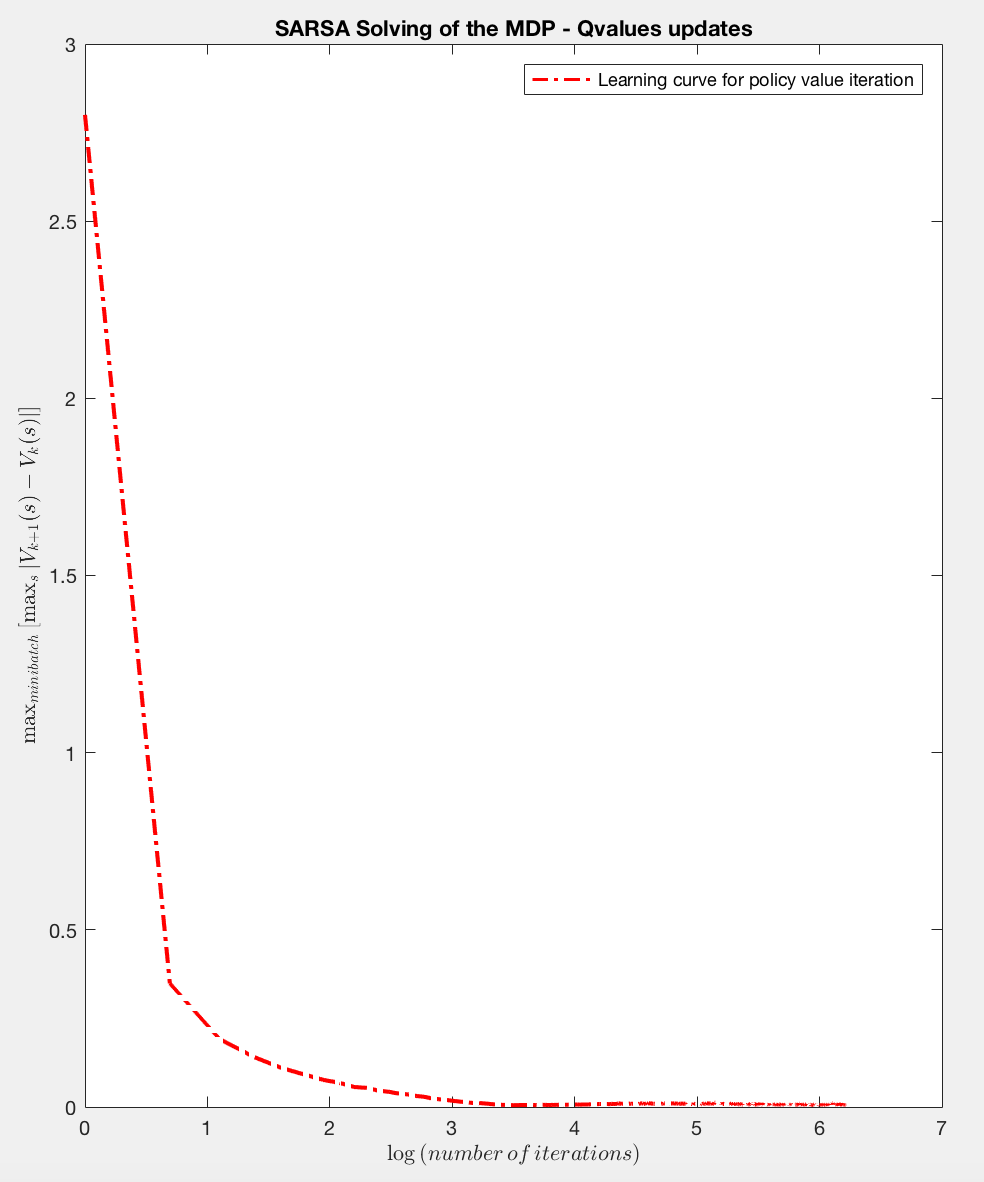
\includegraphics[width=0.9\linewidth]{sarsa_learning_curve_free_grid}
						\caption{Learning curve for SARSA on \emph{free\_grid}}
					\end{minipage}
					\hfill
					\begin{minipage}{0.4\linewidth}
						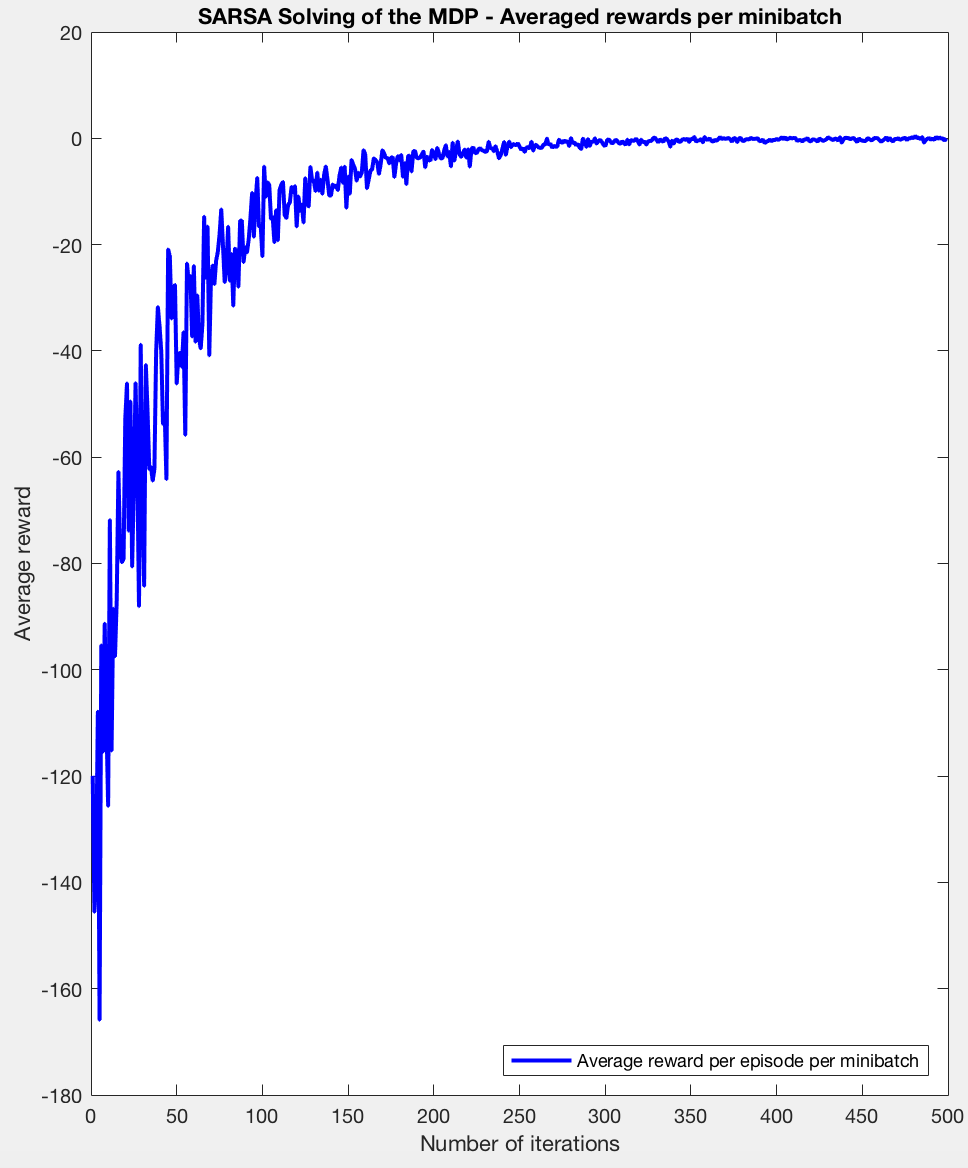
\includegraphics[width=0.9\linewidth]{sarsa_average_rewards_freegrid}
						\caption{Averaged rewards over mini-batch for SARSA on \emph{free\_grid}}
					\end{minipage}
				\end{figure}
				  
			}
			\subsection{Q-learning solving}
			{
			
				\begin{figure}[ht!]
					\begin{minipage}{0.4\linewidth}
						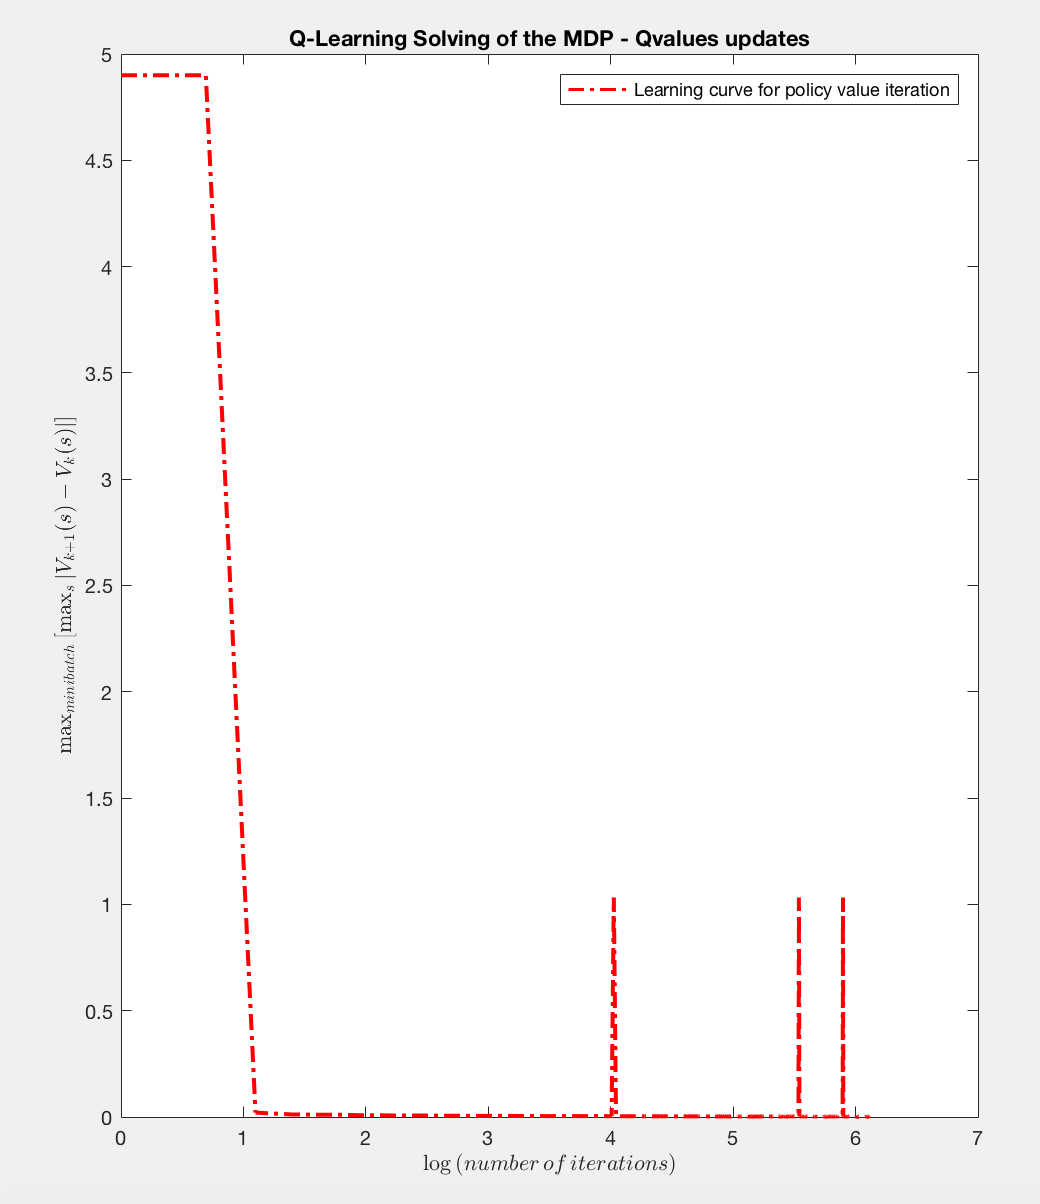
\includegraphics[width=0.9\linewidth]{bargrid_ql_learning_curve}
						\caption{Learning curve for Q-learning on \emph{bar\_grid}}
					\end{minipage}
					\hfill
					\begin{minipage}{0.4\linewidth}
						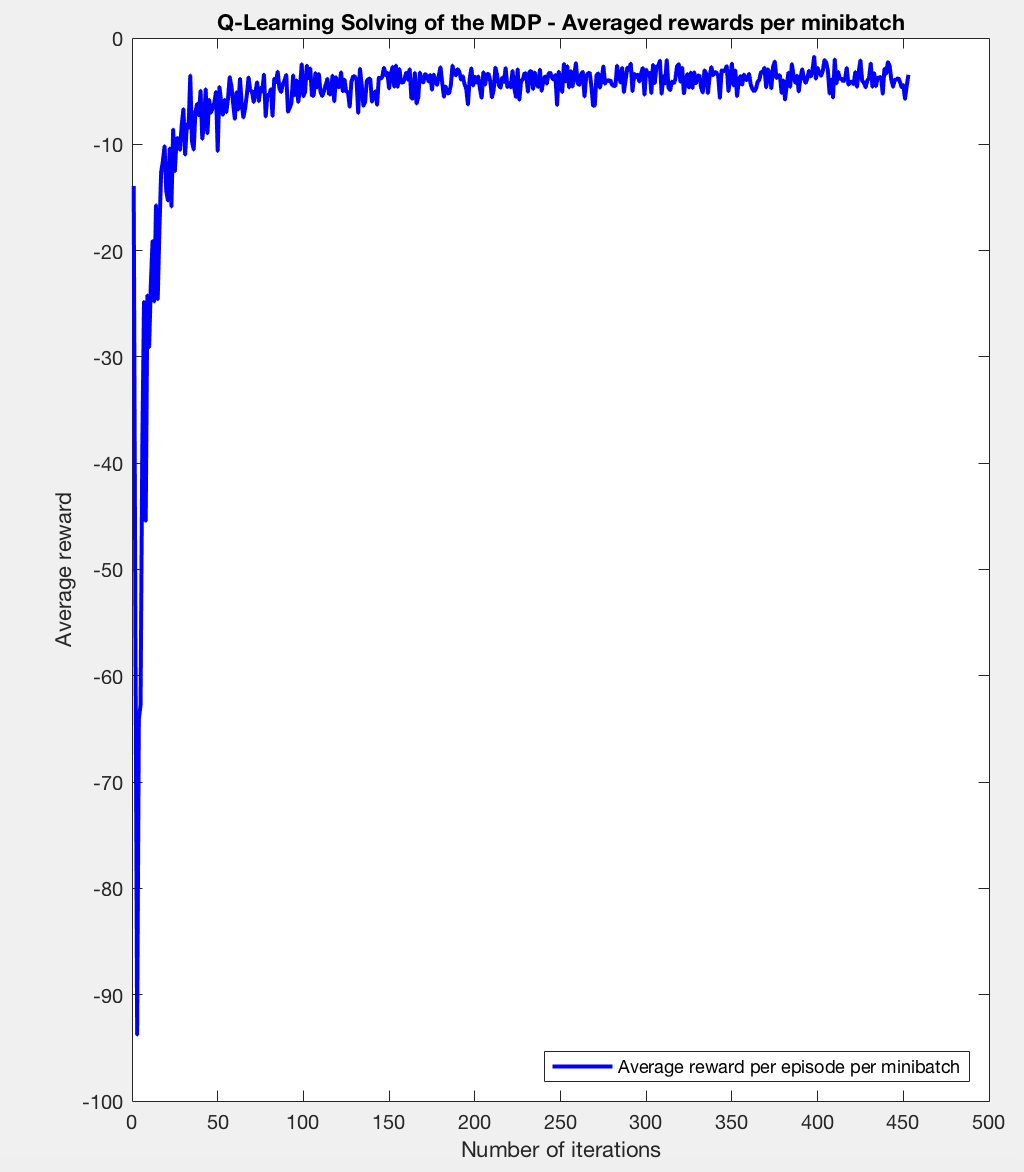
\includegraphics[width=0.9\linewidth]{bargrid_ql_averaged_rewards}
						\caption{Averaged rewards over mini-batch for Q-learning on \emph{bar\_grid}}
					\end{minipage}
				\end{figure}
				\paragraph{} We display here the learning curves for the \emph{bar\_grid} state space using Q-learning. Again, the algorithm manages to learn the optimal policy and the right action-value functions. We use Gibbs sampling for the behavior policy, without any tuning for the temperature (the behavior policy doesn't need to be greedy in limit). The learning curves obtained are given hereinafter.

			}
		}
	}
	
	\chapter{Compliant Reinforcement Learning}
	\chaptermark{Compliant RL}
	{
		 With our approach, we wish to tackle two topics : on one hand, we wish to develop an imitation based learning framework that \emph{accelerates} the learning process. Also, we wish to apply a shifting compliance based behavior so that an agent can overcome an arbitrarily suboptimal teacher.
		
		\section{Principle}
		{
			\paragraph{} We start by making a fairly strong hypothesis to simplify our reasoning. In the following chapters, we will consider that a mentor demonstration provides one recommended action for every state - which is the equivalent of providing one deterministic policy. This somehow out-scopes the case of unique demonstration, but can be understood as a combination of multiple demonstrations.\newline
			Hence, we will consider that a teacher's demonstration is a mapping between the state space $\mathcal{S}$ of the learner and its action set $\mathcal{A}(s)$, $\forall s\in\mathcal{S}$, denoted $\pi_m$ : 
			\begin{equation}
				\begin{aligned}
					\pi_m \, :  \, \mathcal{S} &\to \mathcal{A}\\
						     s &\to a_m(s) 
				\end{aligned}
			\end{equation}
			where $a_m(s)$ is the \emph{recommended action} of the mentor at state $s$. 
			\newline 
			Such an hypothesis isn't trivial, and will be discussed later in this report. The main reason it is considered is that it enables to treat the whole state space in the same way - without having to distinguish regions in the state space that are provided with demonstrations and regions which are not. 
			
			\paragraph{} As discussed earlier in this report, our goal is to mimic the shifting compliance a child can have with respect to its teacher when learning a new skill. Because this implies making choices as to wether follow a recommended action or sample elsewhere in the action space, it is clear that only the action selection (hence the \emph{exploratory policy}) should be impacted by the presence of the mentor. 

			\paragraph{} We will now consider an action selection process based on the teacher's recommandation. We introduce a parameter $p$, that can be understood as a \textbf{confidence measure} in the teacher. The action selection process we chose to follow can be understood as a $p$-greedy action selection with respect to the teacher recommandation and is defined as : 
			\boxedeq{red}
			{
				\forall s\in\mathcal{S}, \quad \pi(s) = \left\{
				\begin{aligned}
					&a_m \, \text{with probability }p \\
					& a \in \mathcal{A}(s) \text{ with probability } (1-p)
				\end{aligned}\right.
				\label{eq::compliant_exploration}
			}
			The learner therefore has two possibilities : follow the teacher with probability $p$, or take its own action, with probability $(1-p)$. This motivates to call $p$ a confidence measure : the greater $p$ is, the more the learner will trust the teacher and follow its recommandation. In the case where the learner decides to take its own action, it samples in its state space through Gibbs softmax sampling, thanks to its current action-value estimates. 
			
			\paragraph{} The purpose of sections (\ref{section::naive_learners}) and (\ref{section::adaptative_learners}) is to provide $p$ with different dynamics through time and evaluate the corresponding performances. 
			
						
			\paragraph{} The updates will follow the SARSA algorithm, and the usual TD(0) updates : $\forall s\in\mathcal{S}, a\in\mathcal{A}(s)$
			\begin{equation}
				Q(s,a) \leftarrow Q(s,a) + \alpha \left[ r + Q(s',a') - Q(s,a) \right]
			\end{equation}
			which are indeed not impacted by the presence of a mentor. Therefore, under the very simple conditions for SARSA to converge to a locally optimal policy (that is, among others, that the exploratory policy is greedy in limit), our algorithms will converge too. 
		}
		\section{Experimental MDP}
		{
			\paragraph{} To test the effectiveness of the solutions we willl propose, we decided to provide ourself with a model that would stay fixed all along the experiments, in order to compare the different algorithms we could come up with. 
			
			\paragraph{} We designed the state space displayed in figure (\ref{fig::maze_display}). In this environment, all black cells are obstacles. They give out highly negative rewards ($r=-10$). Whenever an agent take the action to enter such a cell, it immediately perceives the negative reward but stays in its current cell. The only positive reward is at the middle of the grid ($r=10$), the only terminal state. Any episode starts at one of the corner of the grid (green cells), and every step spent on a non-terminal cell gives out a small negative reward ($r=-0.1$). The transitions are stochastic, with the transition probability model : 
			\begin{equation}
				s' = \left\{ 
					\begin{aligned}
						&a(s) \text{ with proba } 0.95 \\
						&s'' \neq a(s) \text{ otherwise, uniformly sampled}
					\end{aligned}\right.
			\end{equation}
			 
			 \paragraph{} This state space is big enough for the usual algorithms to learn rather slowly, even if they are greatly enhanced by the use of eligibility traces. Also, all tested algorithms (SARSA, Q-learning, SARSA($\lambda$) and Watkins Q($\lambda$)), because they do not perform infinite exploitation / exploration moves, renders slightly suboptimal policies. 
			
			\begin{figure}[ht!]
				\begin{minipage}{0.45\linewidth}
					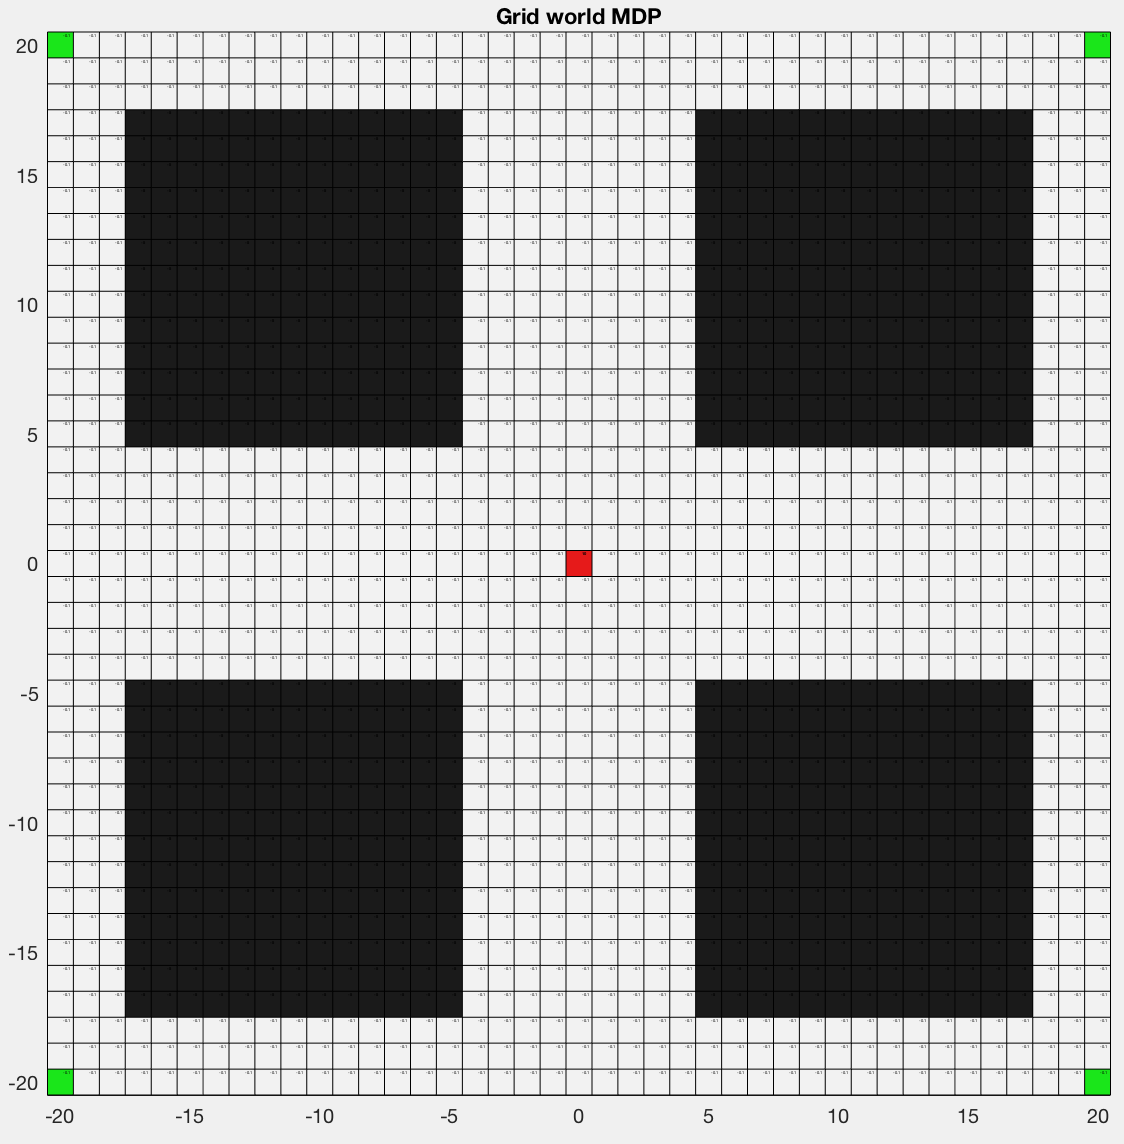
\includegraphics[width=\linewidth]{maze_grid}
					\caption{The \emph{maze\_grid} state space}
					\label{fig::maze_display}
				\end{minipage}
				\hfill
				\begin{minipage}{0.45\linewidth}
					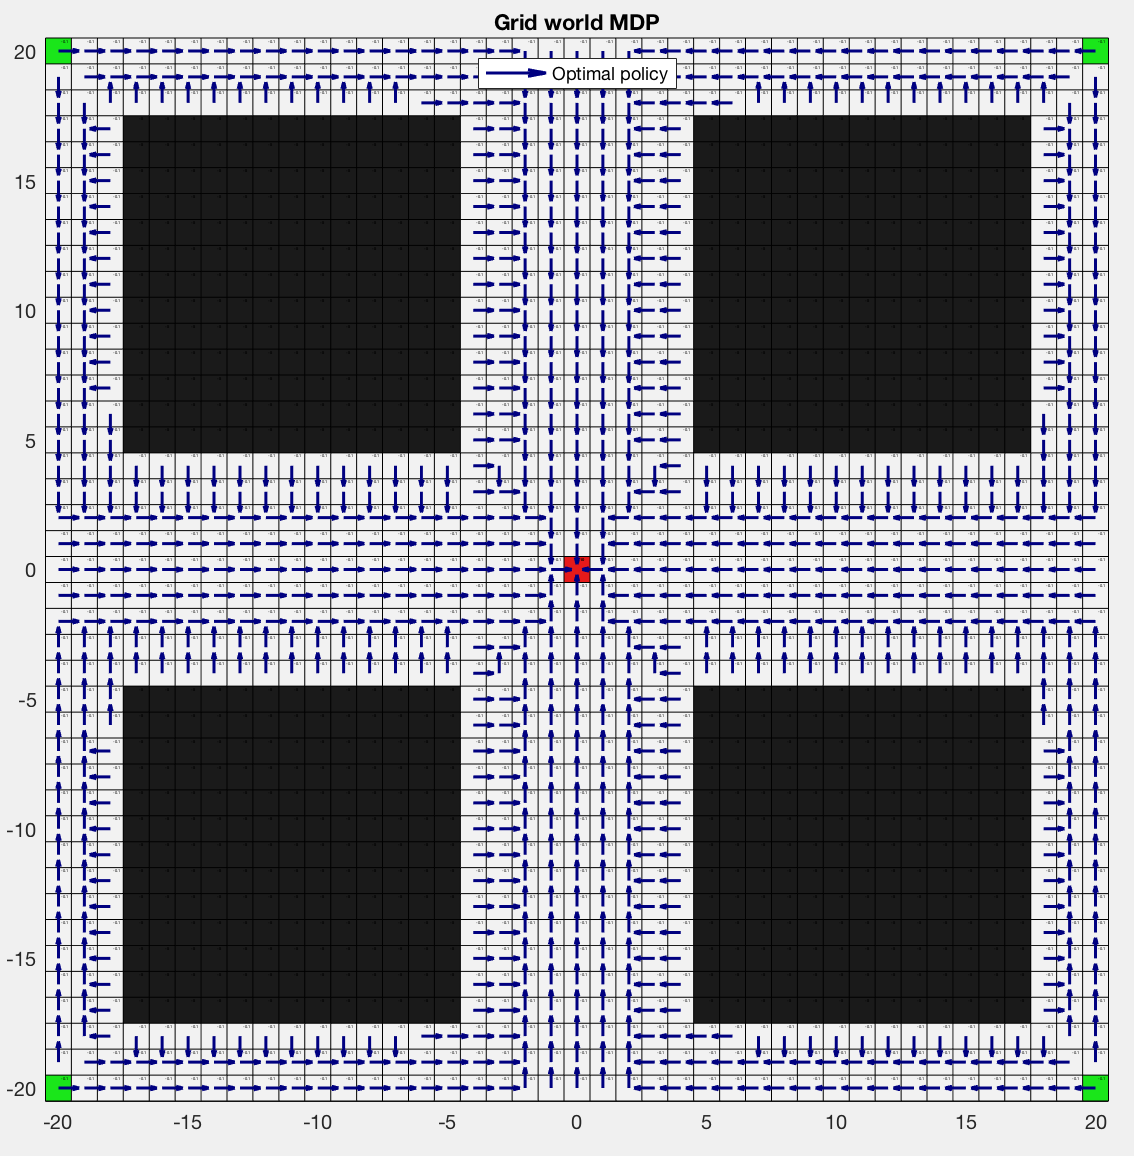
\includegraphics[width=\linewidth]{maze_optimal_policy}
					\caption{Optimal policy, computed with DP}
					\label{fig::maze_optimal_policy}
				\end{minipage}
			\end{figure}
				
			\paragraph{} If we go back at one of our motivating example (robot grasping an object), we could easily draw parallels between such an example and the grid environment we just presented. Indeed, we could imagine a teacher providing a demonstration that borders the obstacle. Because the learner suffers a (slightly) stochastic dynamic, this would indeed be a largely suboptimal solution, since large negative rewards will be likely to occur during the learning. However, the demonstration contains a fairly important information, that is the direction to follow to reach the center of the grid. 
						
			\paragraph{} Figure (\ref{fig::comp_maze}) displays the convergence (expressed as average reward on minibatch) for Qlearning, Sarsa($\lambda$), Sarsa(0) and Watkins Q($\lambda$). By average reward on minibatch, we mean that at every iteration, the reward is average around a given number of trajectories, following the same \emph{exploratory} policy. This allows to reduce the stochasticity of trajectories while learning and give a smoother estimation of how well the algorithm is learning. As a way of comparing them to the optimal and random policies, we also plot the average rewards perceived by the latest along many trajectories. \newline
For all the learning algorithms tested, we used optimistic action-value initialisation to promote exploration. This explains why many negative rewards are perceived in the beginning. 
				
			\begin{figure}
				\begin{center}
					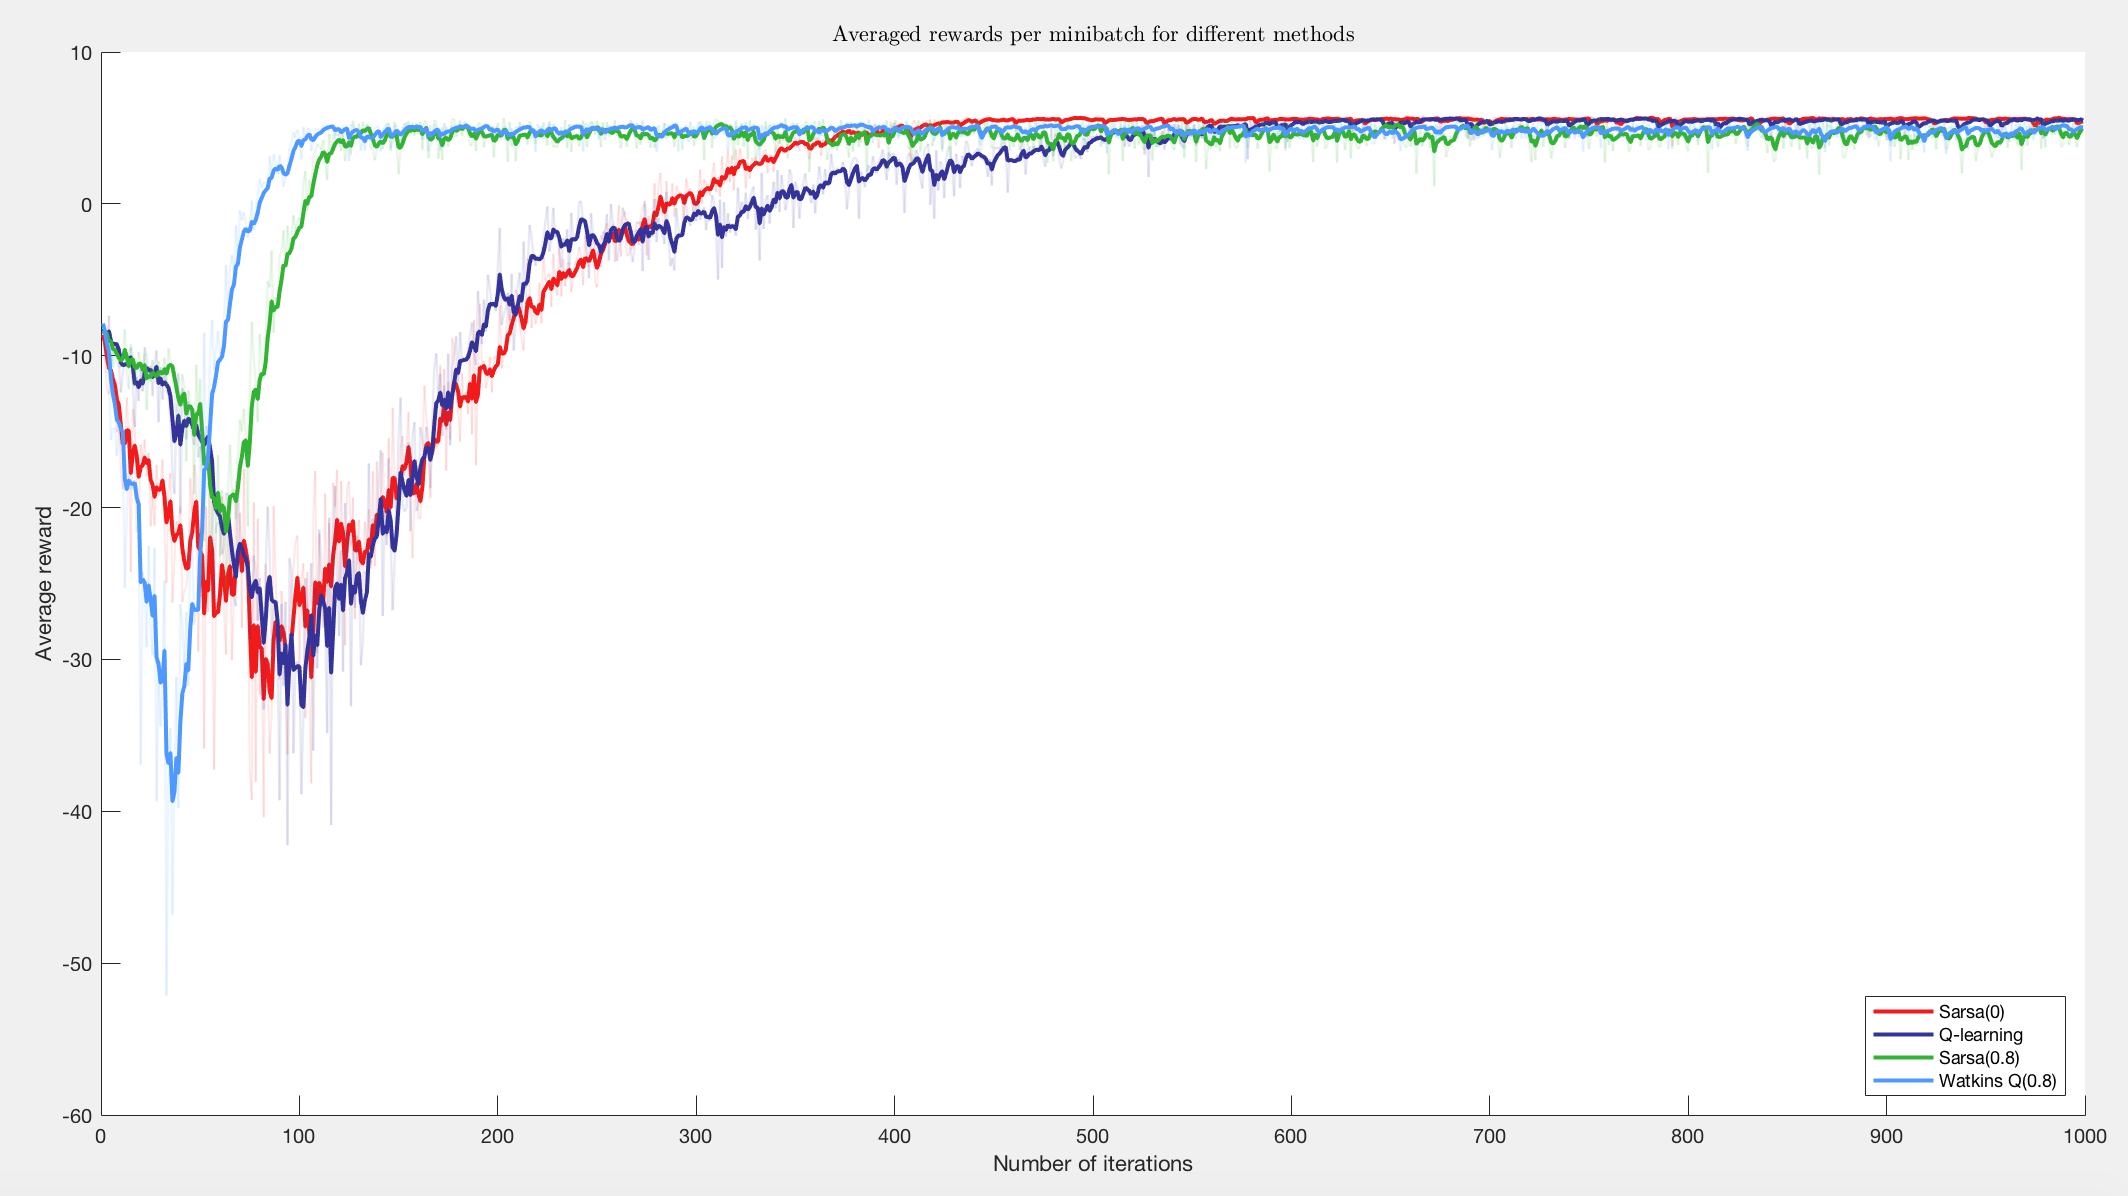
\includegraphics[width=\linewidth]{comp_maze}
					\caption{Average rewards on minibatch for learned policies, optimal policy and random policy.}
					\label{fig::comp_maze}
				\end{center}
			\end{figure}
		}
	\section{Generating mentors}
	{
		\paragraph{} More than giving us an idea how generic reinforcement learning algorithms performs on our sandbox MDP, coding those different methods enables us to \emph{generate mentors of varying sub-optimal levels}. 
		
		\paragraph{} If we consider a SARSA learner (for instance), we can at any time of its learning to generate a deterministic version of the current exploratory policy. This is done by taking its greedy version with respect to its current Q-values estimates. Hence $\forall s\in\mathcal{S}$ : 
		\begin{equation}
			\pi_m(s) = \argmax{a\in\mathcal{A}(s)}{Q(s,a)}
		\end{equation}
		
		\begin{figure}[h!]
			\begin{center}
				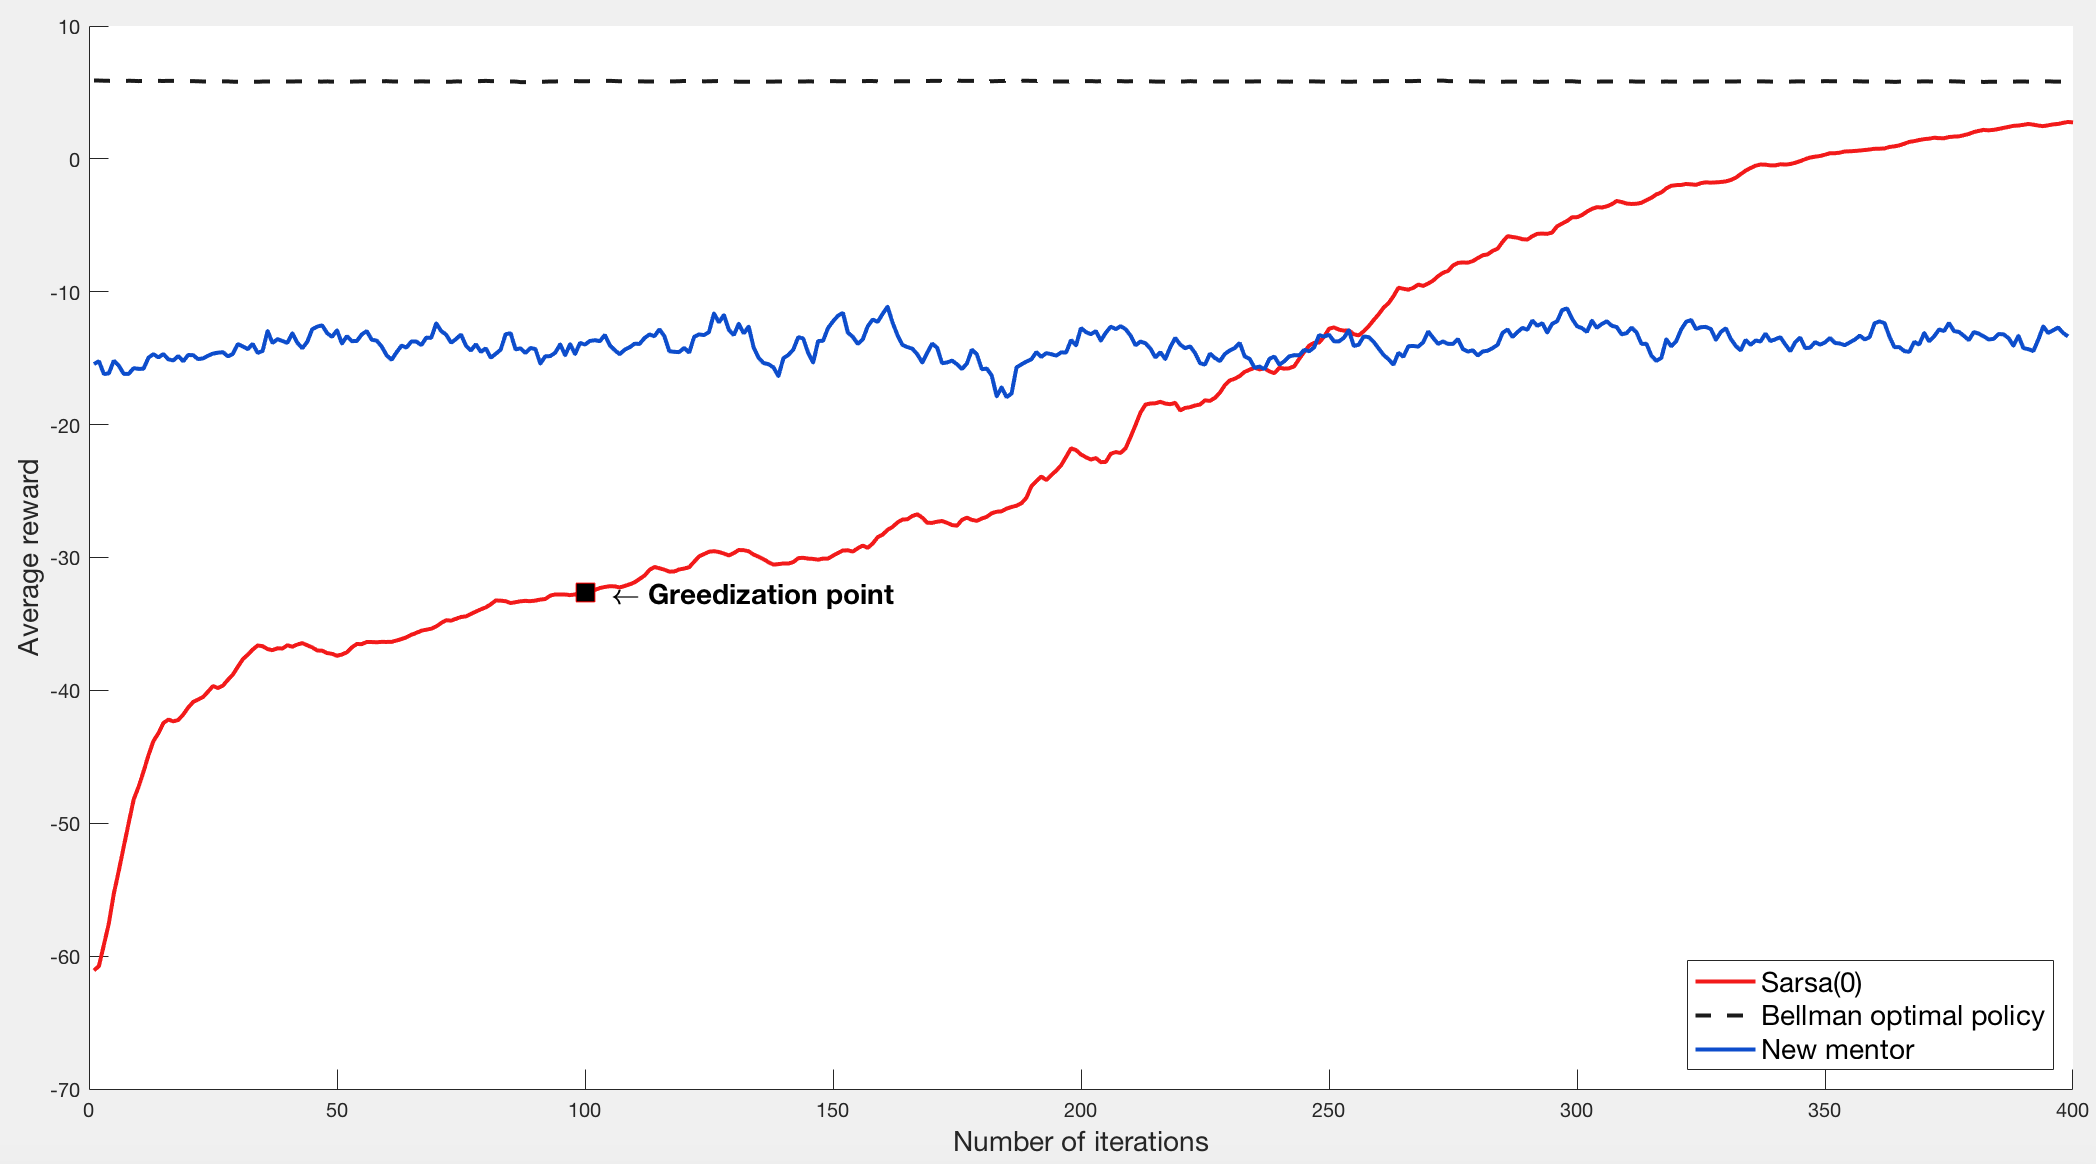
\includegraphics[width=0.8\linewidth]{mentor_gen}
				\caption{Generating a suboptimal mentor from a SARSA learner}
				\label{fig::mentor_gen}
			\end{center}
		\end{figure}
		Such a process is displayed in figure (\ref{fig::mentor_gen}). Because it is now longer stochastic, the mentor is slightly better than the learner it was generated from, but still is clearly suboptimal. This method hence enables us to generate mentor of different optimality levels. 
	}
	\section{Naive learners}
	{
		\label{section::naive_learners}
		\subsection{Constant compliance}
		{
			\paragraph{} In the context of the action-selection described in (\ref{eq::compliant_exploration}), we decided to first implement a fairly naive method. It consists in following the teacher's recommandation with a \textbf{constant} confidence term $p$. Therefore, the learner \emph{complies} with the teacher with probability $p$, and decide to choose its own action (that \textbf{could include} $\boldsymbol{a_m}$) with probability $1-p$. The softmax sampling used when discarding a recommandation is tuned by a decaying temperature coefficient, making it greedy in limit.
			
			\paragraph{} The figures (\ref{fig::comp_opt_verynaive}) and (\ref{fig::comp_subopt220_verynaive}) display the learning obtained (cumulated rewards averaged over mini-batches) when fed with, respectively, the optimal policy for the MDP and a slightly suboptimal one. 
			
			\begin{figure}[ht!]
				\begin{minipage}{0.5\linewidth}
					\begin{center}
						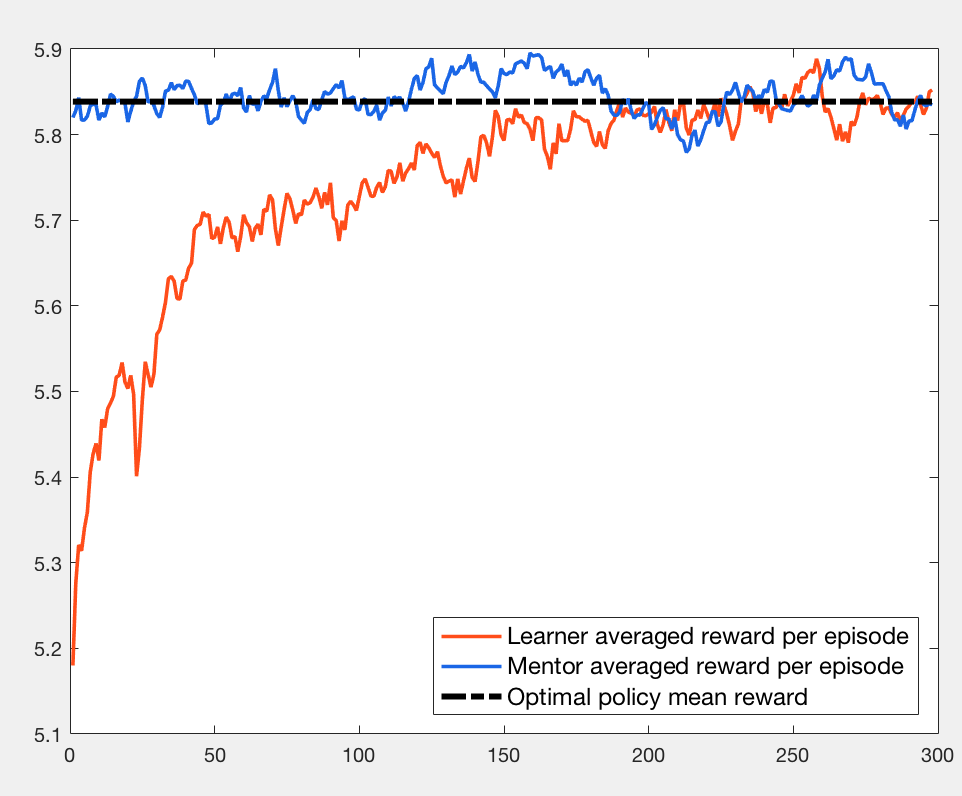
\includegraphics[width=0.9\linewidth]{very_naive_opt}
						\caption{Constant compliance learning, $p=0.9$, with the optimal mentor}
						\label{fig::comp_opt_verynaive}
					\end{center}
				\end{minipage}
				\begin{minipage}{0.5\linewidth}
					\begin{center}
						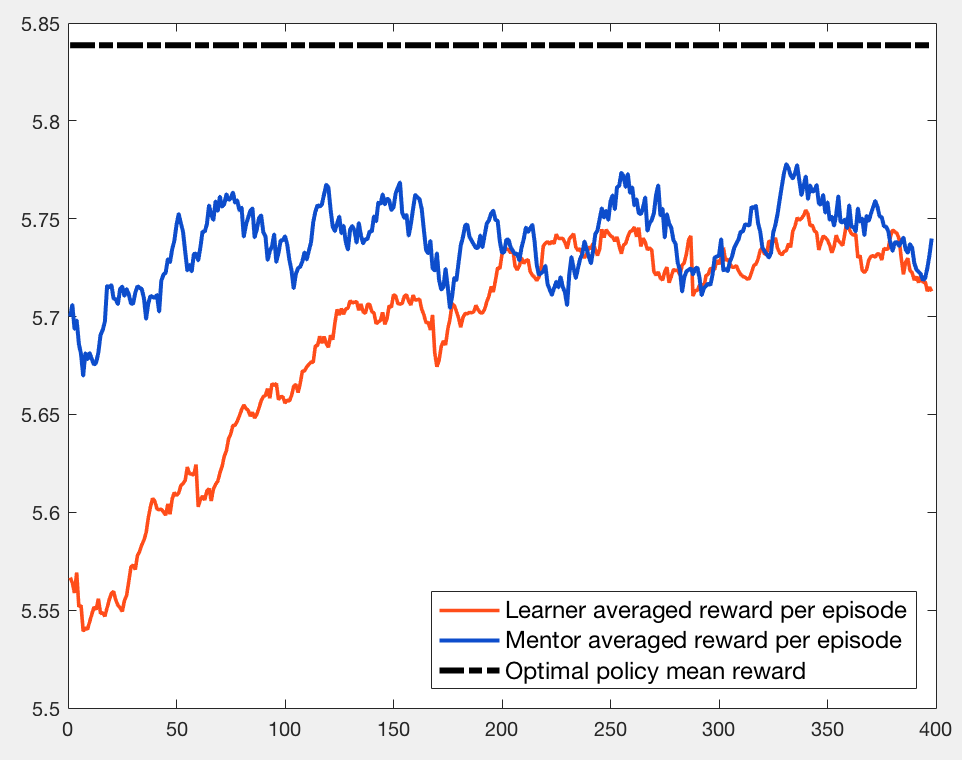
\includegraphics[width=0.9\linewidth]{very_naive_200}
						\caption{Constant compliance learning, $p=0.9$, with a slightly suboptimal mentor}
						\label{fig::comp_subopt220_verynaive}
					\end{center}
				\end{minipage}
			\end{figure}
	
			\paragraph{} Figure (\ref{fig::comp_opt_verynaive}) shows that from its exploration, the learner is able to quickly learn his way thanks to the optimal mentor. As expected, it eventually follows the mentor's action, wether it complies or not, since the recommended action holds the best action-values. On the other hand, as shown in figure (\ref{fig::comp_subopt220_verynaive}), the high confidence the learner initially have in its mentor prevents it from reaching optimal performance, and the policy its renders actually mimic its mentor suboptimal one. Still, one could expect the learned policy to be slightly better than its suboptimal teacher's one, even if not optimal. However, achieving this comes with a lot of effort in the tuning of $p$ and of the softmax distribution temperature decrease coefficient. 
	
			\begin{figure}[ht!]
				\begin{center}
					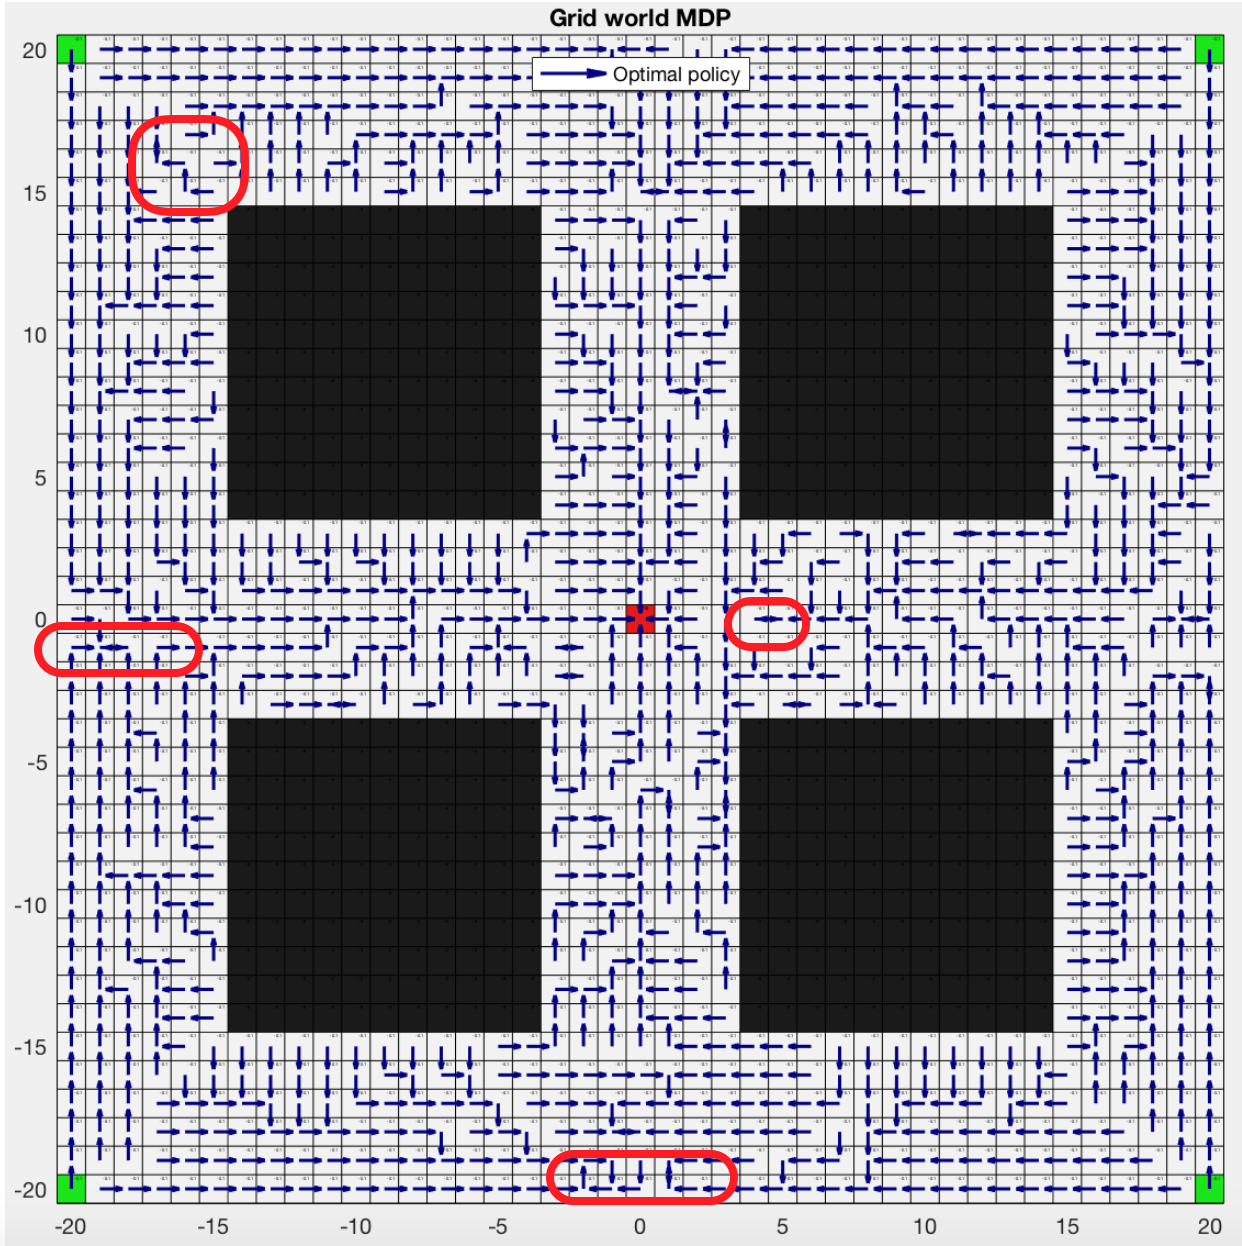
\includegraphics[width=0.7\linewidth]{subopt_policy_block}
					\caption{An exemple of suboptimal mentor policy that doesn't always lead to the positive reward}
					\label{subopt_policy_block}
				\end{center}
			\end{figure}
			
			\paragraph{} This remark actually pinpoints a major downside of this method, that is the need of fine tuning of the parameter $p$. But obviously, there is even a bigger downside, that becomes a major game killer when dealing with largely suboptimal mentors. Indeed, some mentors can be suboptimal enough to only show a good direction of exploitation, but not be able to reach the target. . Figure (\ref{subopt_policy_block}) displays such a policy, where the mentor's policy creates loops and does not always leads to the positive reward.  \newline. 
			Applying the latest method with such a teacher is fatal for the learning, as the learner discovers that following the mentor's action yields largely negative rewards, but is not able to bypass them as it keeps a constant confidence in its teacher. This leads the learner to build up low Q-values in the directions recommended by the mentor, and to try to follow an opposite path. This is highly counter-productive since the mentor still gives the right exploration direction. 
		
		\subsection{Vanishing compliance }
		{
			\paragraph{} One of the downside of the constant compliance approach is that the exploratory behavior is always biased by the mentor's recommandation. This breaks the need of this policy to be \emph{greedy in limit} (which is a specification for SARSA algorithm to converge). In the case of a sub-obptimal mentor, this means that the optimal behavior could never be reached. 
			
			\paragraph{} We now decide to comply with the need to be greedy in limit. Therefore, we decide to set $p$ to be \emph{constantly decreasing along the learning procedure} : 
			\begin{equation}
				p_{t+1} = \beta p_{t}
			\end{equation}
			with $\beta < 1$. As before, the temperature of the Gibb's softmax sampling also goes to $0$ as the learning goes on. 
			
			\paragraph{} The action-selection is therefore biased by the mentor's recommandation in the beginning of the learning only, and slowly decides to take its own choices, based on its current Q-values estimates. This approach sounds more promising as the learner is more likely to quickly discover the location of high rewards (following the teacher policy with $p$ close to 1), and will then makes it own exploration along those trajectory, to end up in a setting where the teacher's actions are now longer considered. 
		
			\begin{figure}[ht!]
				\begin{minipage}{0.5\linewidth}
					\begin{center}
						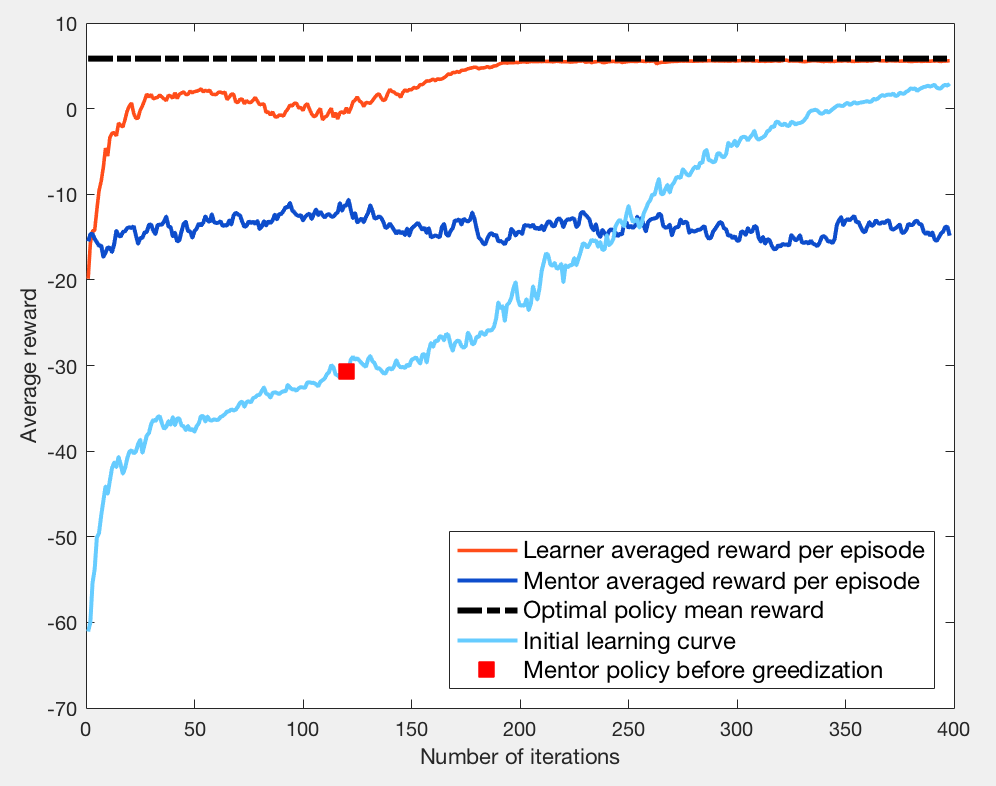
\includegraphics[width=0.95\linewidth]{comp_naive_compliance_120}
						\caption{Vanishing compliance, $\beta = 0.99$}
						\label{fig::comp_naive_compliance_120}
					\end{center}
				\end{minipage}
				\begin{minipage}{0.5\linewidth}
					\begin{center}
						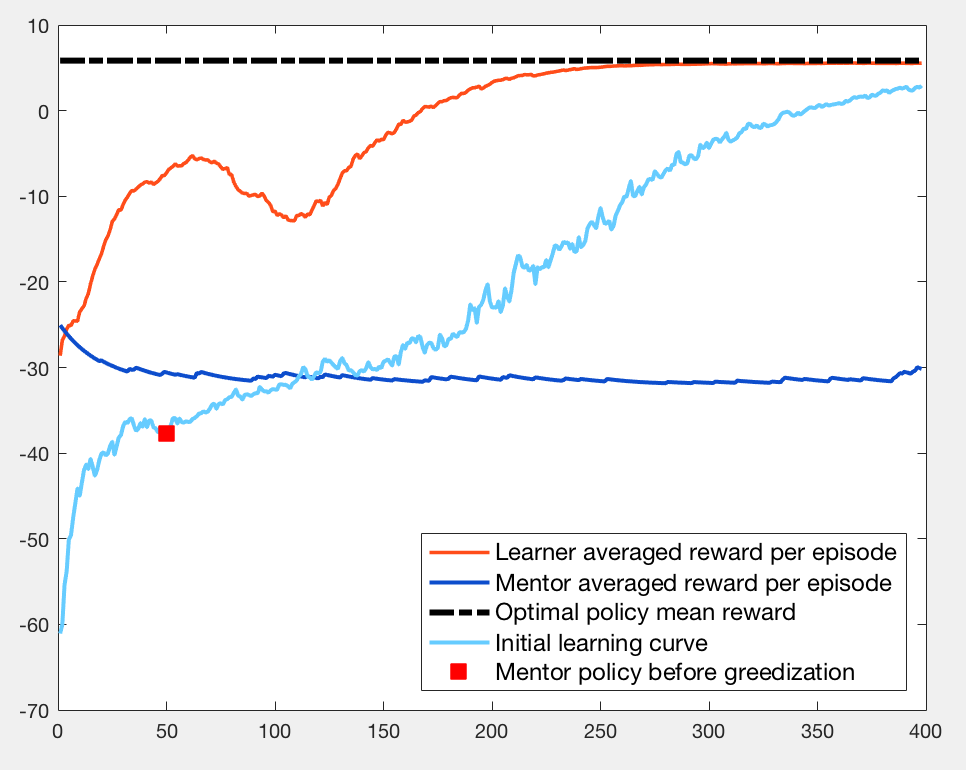
\includegraphics[width=0.95\linewidth]{comp_naive_compliance_50}
						\caption{Vanishing compliance, $\beta = 0.97$}
						\label{fig::comp_naive_compliance_50}
					\end{center}
				\end{minipage}
			\end{figure}
			
			\paragraph{} Figures (\ref{fig::comp_naive_compliance_120}) and (\ref{fig::comp_naive_compliance_50}) display the result on two sub-optimal policies, that were derived from the Q-values learned at a given moment (denoted through a red square) in a learning process. They show that with this approach, while the learner is compliant with the teacher, it steadily increases its accumulated reward thanks to its exploratory actions. However, it then comes to a plateau (or even an undershoot) when the guidance by the teacher becomes too weak as $p$ reaches a critical level. The learner then mostly relies on its exploratory actions (which volatility are guided by its temperature coefficient) to explore new regions of the state space. Once it has somehow learnt the action value function related to this part of its state space, and as its temperature goes down, the learner's accumulated reward goes up until it reaches the level of the optimal policy. 

		}		
		
		\paragraph{} If this approach seems to work relatively well, there are still some critical downsides to it. First of all, a lot of tuning is required in order to find the hyper-parameters ($p_0$, $\beta$, temperature evolution, ..) that lead to a fast learning. Also, there is an undershoot in the learning that seems to slow it down, due to the exploring phase that happens when $p$ becomes too low.  Such exploration could be avoided or reduced if the learner is able to figure out quickly that indeed, the mentor was right in its recommandation.
	}
	
	\section{Adaptative compliance learners}
	{	
		\label{section::adaptative_learners}
		\paragraph{} Up to this point, it makes sense to somehow \emph{learn} the optimal value of the confidence parameter $p$, so that we don't have to manually tune its evolution, and so that it can store how right the teacher recommandations are. Ideally, we would like $p$ to be near $0$ when the teacher provide a suboptimal action and $1$ when the recommended action is sampled from the optimal policy. The underlying problem is therefore to infer the optimality of the teacher in different regions of the state space. 
		
		\paragraph{}We hereinafter describe two methods which attempt to do so. Their respective experimental results as well as further discussion will be found in chapter (\ref{chap::res}).  
		
		\subsection{Implicit $\beta$-compliance}
		{
			\paragraph{}  Let us define the \emph{confidence} term $p$ locally for every state of the state space. For each $s\in\mathcal{S}$, $p(s)$ is given a Beta prior : $p(s)\sim \beta(\alpha(s),\beta(s))$ and represents the initial trust we have in a mentor's recommandation at state $s$. The initial values $\alpha_0$ and $\beta_0$ define the initial prior belief we have over $p$ (for instance, $\alpha=0.5$ and $\beta = 0.055$ define a prior belief that the teacher is most probably right). 
			
			\paragraph{} As in before, we perform a $\color{red}p$\textcolor{red}{\emph{-greedy policy}} with respect to the teacher recommandation : 
			\begin{equation}
				\forall s\in\mathcal{S}, \quad \pi_p(s) = 
					\left\{ 
					\begin{aligned}
						&a_m \text{ with probability } p(s) \\
						& a\in\mathcal{A}(s) \text{ with probability } (1-p(s))
					\end{aligned}
					\right. 
			\end{equation}
		
			\paragraph{} The following describe how we wish to learn the value of $p(s)$, $\forall s\in\mathcal{S}$. Based on the $5$-tuple $(s,a,r,s',a')$ obtained thanks to the action selection process we just described, we compute at every step the following temporal difference value : 
			\begin{equation}
				\delta_t = r + \gamma Q(s',a') - Q(s,a_m)
			\end{equation}
			which compares, \emph{in average}, the advantage (our drawback) of following the state-action pair $(s,a)$ rather than the one indicated by the teacher, according to the current Q-values estimates. 
		
			\paragraph{} We then apply the following update rule to $p(s)$ : 
			\begin{equation}
				\label{eq::update_rule}
				\begin{aligned}
					\alpha_t(s) &\leftarrow \alpha_t(s) +  \mathds{1}_{a=a_m}\delta_t \eps_t\\
					\beta_t(s) &\leftarrow \beta_t(s) +   \mathds{1}_{a\neq a_m}\delta_t \eps_t
				\end{aligned}
			\end{equation}
			The intuition behind this update rule is simple : if we see that the expected return for the mentor action increases (resp. decreases), then we increase (resp. decrease) $\alpha$ which results in a shift of $p$ toward a larger (resp. smaller) confidence. A similar reasoning holds for the $\beta$ term.  $\eps_t$ is the update rule's learning rate, which value and dynamic will be discussed later. 
		
		}
	
		\subsection{Explicit compliance}
		{
			\paragraph{} We consider here a somewhat similar approach, where our listen versus discard exploration policy is computed according to the current estimated values of the actions \emph{'listen'} and \emph{'discard'}. Let us introduce the action spaces : 
			\begin{equation}
				\forall s\in\mathcal{S}, \, \mathcal{A}_c(s) = \left\{ 'listen', \, 'discard'\right\}
			\end{equation}
			to which we assign the action values $Q_c(\cdot,l)$ and  $Q_c(\cdot,d)$ (where $'l'$ denotes the action of listening and $'d'$ the action of discarding the teacher recommendation). 
			
			\paragraph{} The exploration is done by computing a soft policy derived from $\{Q_c(s,l), Q_c(s,d)\}$ for all $s\in\mathcal{S}$. We do this using a Gibbs softmax distribution, which yields : 
			\begin{equation}
				\forall s \in\mathcal{S}, \quad \pi_c(s) = 
					\left\{
						\begin{aligned}
							&'l' \text{ with probability } p=\sigma\left(\frac{Q_c(s,l) - Q_c(s,d)}{\tau} \right) \\
							& 'd'  \text{ with probability } 1-p
						\end{aligned}
					\right.
			\end{equation}
			where $\sigma(\cdot)$ is the logistic sigmoid and $\tau$ is a temperate coefficient decreasing to $0$ (greedy policy in limit). 
			
			\paragraph{} After each SARSA update, we also make the following update : 
			\begin{equation}
				\label{eq::av_update_rule}
				\left\{
				\begin{aligned}
					&Q_c(s,l) \leftarrow  \beta Q_c(s,l) + (1-\beta)Q(s,a_m) \\
					&Q_c(s,d) = \beta Q_c(s,d) + (1-\beta)\max_{a\neq a_m} Q(s,a) 
				\end{aligned}
				\right.
			\end{equation}
			with $\beta >0$ the update rule's learning rate. 
			\paragraph{} We can introduce some prior confidence in the teacher by setting, $\forall s\in\mathcal{S}$ : 
			\begin{equation}
				Q^0_c(s,l) - Q^0_c(s,d) = \log\{\frac{p}{1-p}\}
			\end{equation}
			where $p$ is the retained probability of initially choosing to listen to the teacher. 
			}
		}	
	}
	
	\chapter{Results}
	{
		\label{chap::res}
	
		\section{Implicit $\beta$-compliance}
		{
			\paragraph{} We hereinafter give some practical considerations for the implicit $\beta$-compliance and explicit compliance methods, and discuss the experimental results we obtained. 
			\subsection{Practical considerations}
			{
				\paragraph{} One of the main specification of the SARSA learning paradigm is that the exploration policy must be \emph{greedy in limit} so that a fixed point can emerge (hopefully the set of Q-values related to the optimal policy). In an actor-critic approach, the usual way to bring the \emph{critic} term in a stationary regime is to modify its learning rate to take the probability of taking an action into account (see \cite{Sutton98a}). \newline
				This is the approach we chose in order to pick the learning rate $\eps_t$ of the update rule (\ref{eq::update_rule}), which now becomes : 
			\begin{equation}
				\begin{aligned}
					\alpha_t(s) &\leftarrow \alpha_t(s) +  \mathds{1}_{a=a_m}\gamma \delta_t p(s)\\
					\beta_t(s) &\leftarrow \beta_t(s) +   \mathds{1}_{a\neq a_m}\gamma \delta_t (1-p(s))
				\end{aligned}
			\end{equation}
			with $\gamma >0$. This update rule can still be simplified, by approximating $p$ by its mean value, which gives the update rule that we applied in practice : 
			\boxedeq{red}
			{
				\begin{aligned}
					\alpha_t(s) &\leftarrow \alpha_t(s) +  \mathds{1}_{a=a_m} \frac{\gamma \alpha_t(s)}{\alpha_t(s) + \beta_t(s) }\delta_t \\
					\beta_t(s) &\leftarrow \beta_t(s) +   \mathds{1}_{a\neq a_m} \frac{\gamma \beta_t(s) }{\alpha_t(s) + \beta_t(s) } \delta_t
				\end{aligned}
			}
			This ensures us that we will direct the update toward a fixed point, and end up with a greedy policy (in limit). 
			
			\paragraph{} In this method, $p$ is given a Beta prior distribution. To perform the action selection, we would therefore need to sample $p(s)$ from its current distribution, and then sample a Bernoulli random variable of parameter $p(s)$. Assuming that the Beta distribution is sharply peaked around its mean (which we will guarantee by choosing an appropriate prior and learning rate $\gamma$). Then $p(s)$ can be approximated by its mean value $\E{p(s)} = \displaystyle\frac{\alpha(s)}{\alpha(s) + \beta(s)}$. We therefore only need to sample a Bernoulli random variable of parameter $\E{p(s)}$ at every state to complete the action selection process. 
			
			\paragraph{} The tuning that needs to be done is therefore left to $\gamma$, the prior and the temperature. In this framework, tuning is made much simpler and one only has to check that the updates are of the same order of magnitude with the prior (in order for the posterior distribution to adapt to observations, but also to retain the memory of the prior). 
			}
			\subsection{Results}
			{
				\paragraph{} Figures (\ref{fig::ac_il_subopt_120}) and (\ref{fig::ac_il_subopt_50}) show the learning curves for an agent using the $\beta$-compliance, with two different suboptimal teachers. As before, both of them were generated by observing the Q-values of a "normal" learner (without mentor) and by creating the greedy policy with respect to them.  
				
				\begin{figure}[ht!]
					\begin{minipage}{0.5\linewidth}
						\begin{center}
							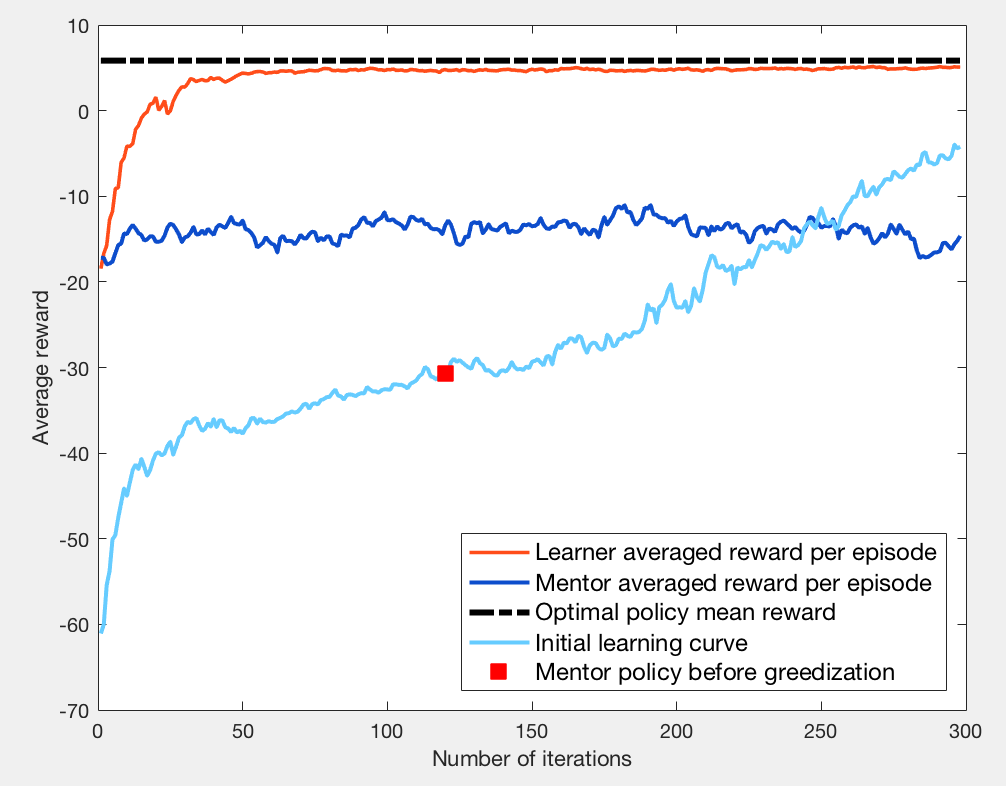
\includegraphics[width=0.95\linewidth]{ac_il_subopt_120}
							\caption{Actor-critic learnt compliance learning curve for }
							\label{fig::ac_il_subopt_120}
						\end{center}
					\end{minipage}
					\begin{minipage}{0.5\linewidth}
						\begin{center}
							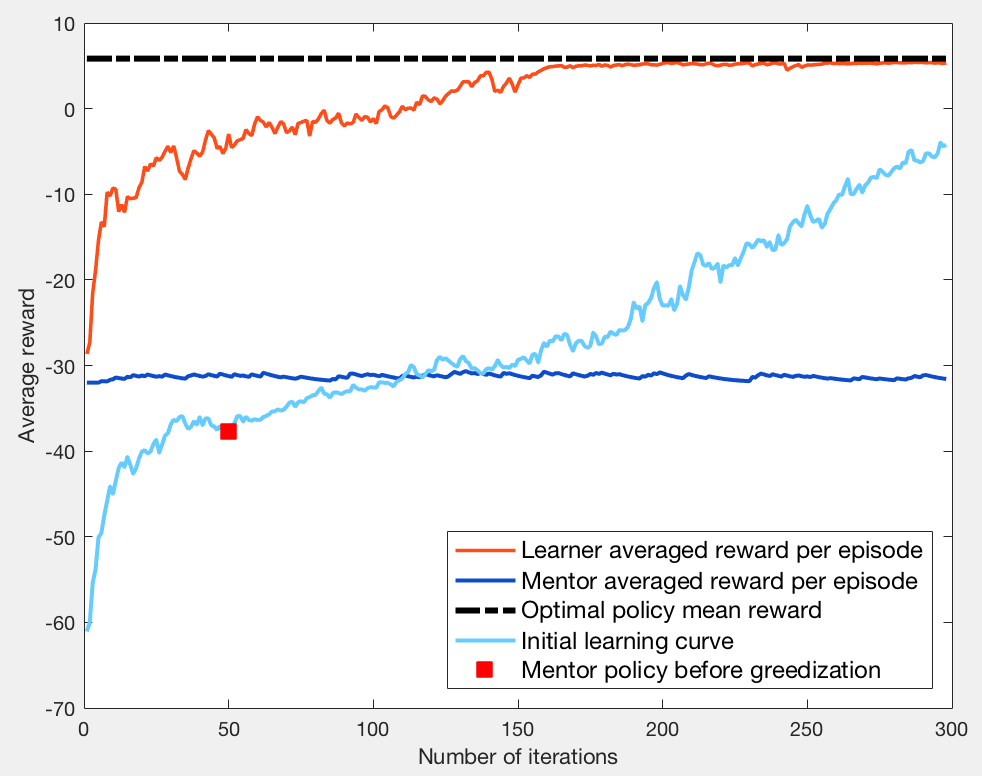
\includegraphics[width=0.95\linewidth]{ac_il_subopt_50}
							\caption{Actor-critic learnt compliance learning curve}
							\label{fig::ac_il_subopt_50}
						\end{center}
					\end{minipage}
				\end{figure}
				
			\paragraph{} The first remark we can make is that by learning the confidence, we were able  to avoid the undershoot that we observed for the vanishing compliance method (see figures (\ref{fig::comp_naive_compliance_120}) and (\ref{fig::comp_naive_compliance_50})). This results in a faster learning and better behaving learning curves. The different methods will be further compared in (\ref{sec_method_comp}). 
			}
			\subsection{Discussion}
			{
				\paragraph{} It would be interesting to see what is the \emph{posterior distribution} of the $p(s)$ , $s\in\mathcal{S}$. We expect our final policy to be greedy, and hence the posterior distribution of the compliance term to be sharply peaked around $0$ or $1$, with proportion given by how good the mentor is.. Figures (\ref{fig::post_mean_120}) and (\ref{fig::post_mean_50}) display the histogram of the repartition of the mean of $p(s)$, $s\in\mathcal{S}$ (again, we approximate the Beta distribution by its mean to have an understandable visualization), for two different mentors (figure (\ref{fig::post_mean_120}) uses the mentor of (\ref{fig::ac_il_subopt_120}) and figure (\ref{fig::post_mean_50}) the mentor of (\ref{fig::ac_il_subopt_50})) . As expected, most of the means are either close to $0$ and $1$, and they are more means close to 0 (poor confidence) when using the second mentor that is far worse than the first. 
				
				\begin{figure}[ht!]
					\begin{minipage}{0.5\linewidth}
						\begin{center}
							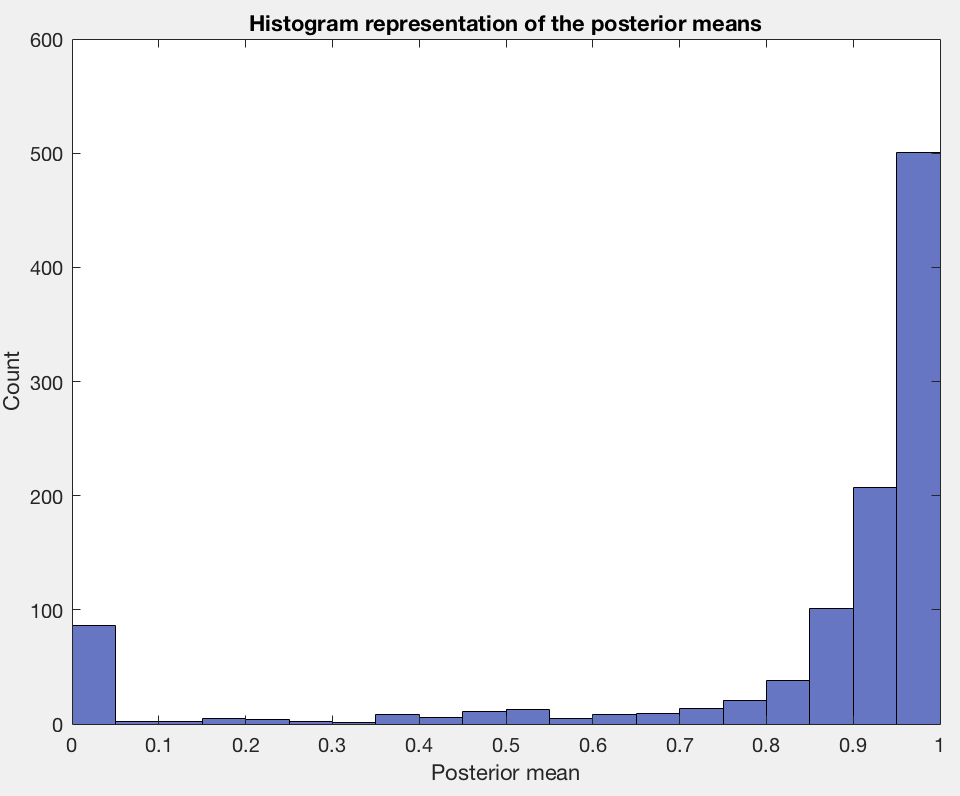
\includegraphics[width=0.95\linewidth]{post_mean_120}
							\caption{Histogram representation of the posterior means for a suboptimal teacher}
							\label{fig::post_mean_120}
						\end{center}
					\end{minipage}
					\begin{minipage}{0.5\linewidth}
						\begin{center}
							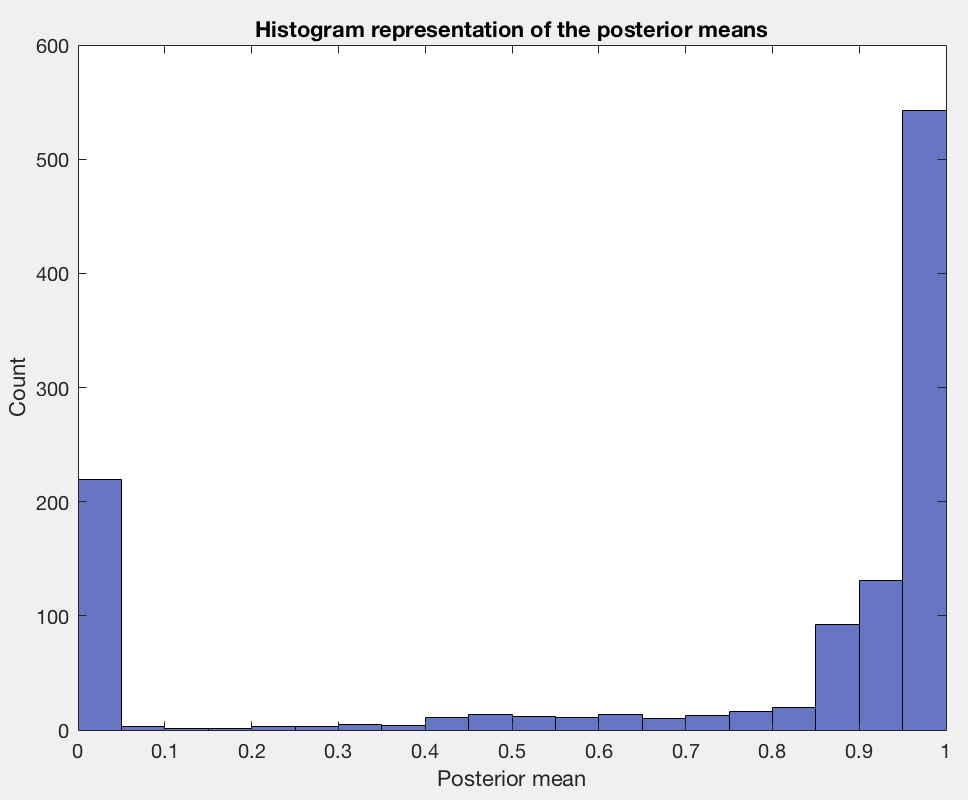
\includegraphics[width=0.95\linewidth]{post_mean_50}
							\caption{Histogram representation of the posterior means for a even more suboptimal teacher}
							\label{fig::post_mean_50}
						\end{center}
					\end{minipage}
				\end{figure}
				
				\paragraph{} Also, to better understand how this algorithm works, it would be interesting to visualize the areas where the learner rejects or listen to its mentor. We expect the learner to discard the mentor's recommandations where those are wrong, and to trust its mentor where it is right. Figures (\ref{fig::heatmap_confidence_120}) and (\ref{fig::heatmap_confidence_50}) display, for two different mentors (the same two ones as we just used), the mentor's policy and the heat-map of the confidence the learner as acquired with respect to its teacher's recommandation at the end of the learning. 
				
				 \begin{figure}[ht!]
					\begin{minipage}{0.5\linewidth}
						\begin{center}
							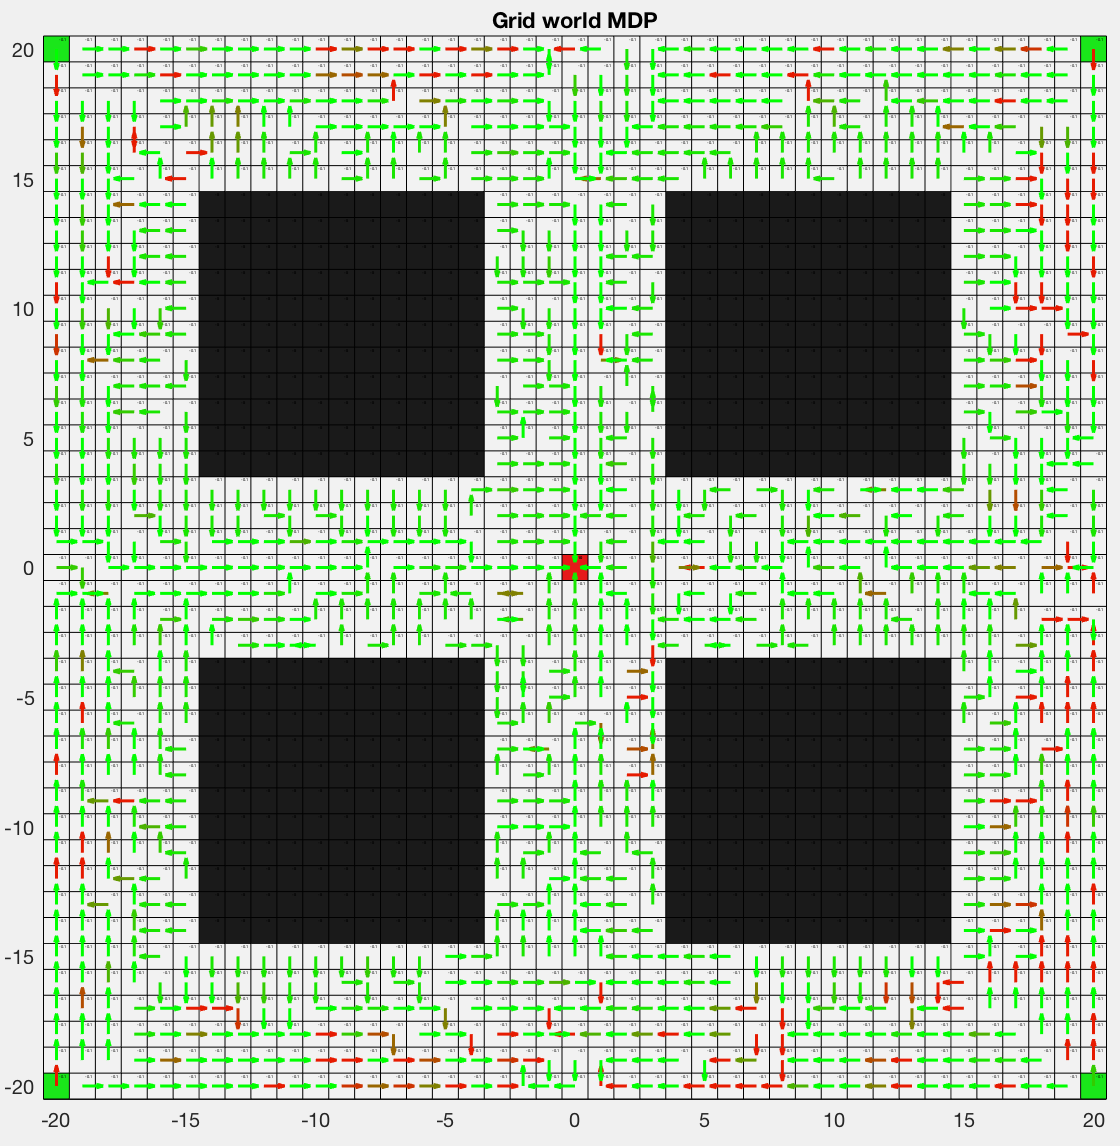
\includegraphics[width=0.95\linewidth]{heatmap_confidence_120}
							\caption{Learnt confidence : green arrows show near 1 posterior mean, red arrows near 0}
							\label{fig::heatmap_confidence_120}
						\end{center}
					\end{minipage}
					\begin{minipage}{0.5\linewidth}
						\begin{center}
							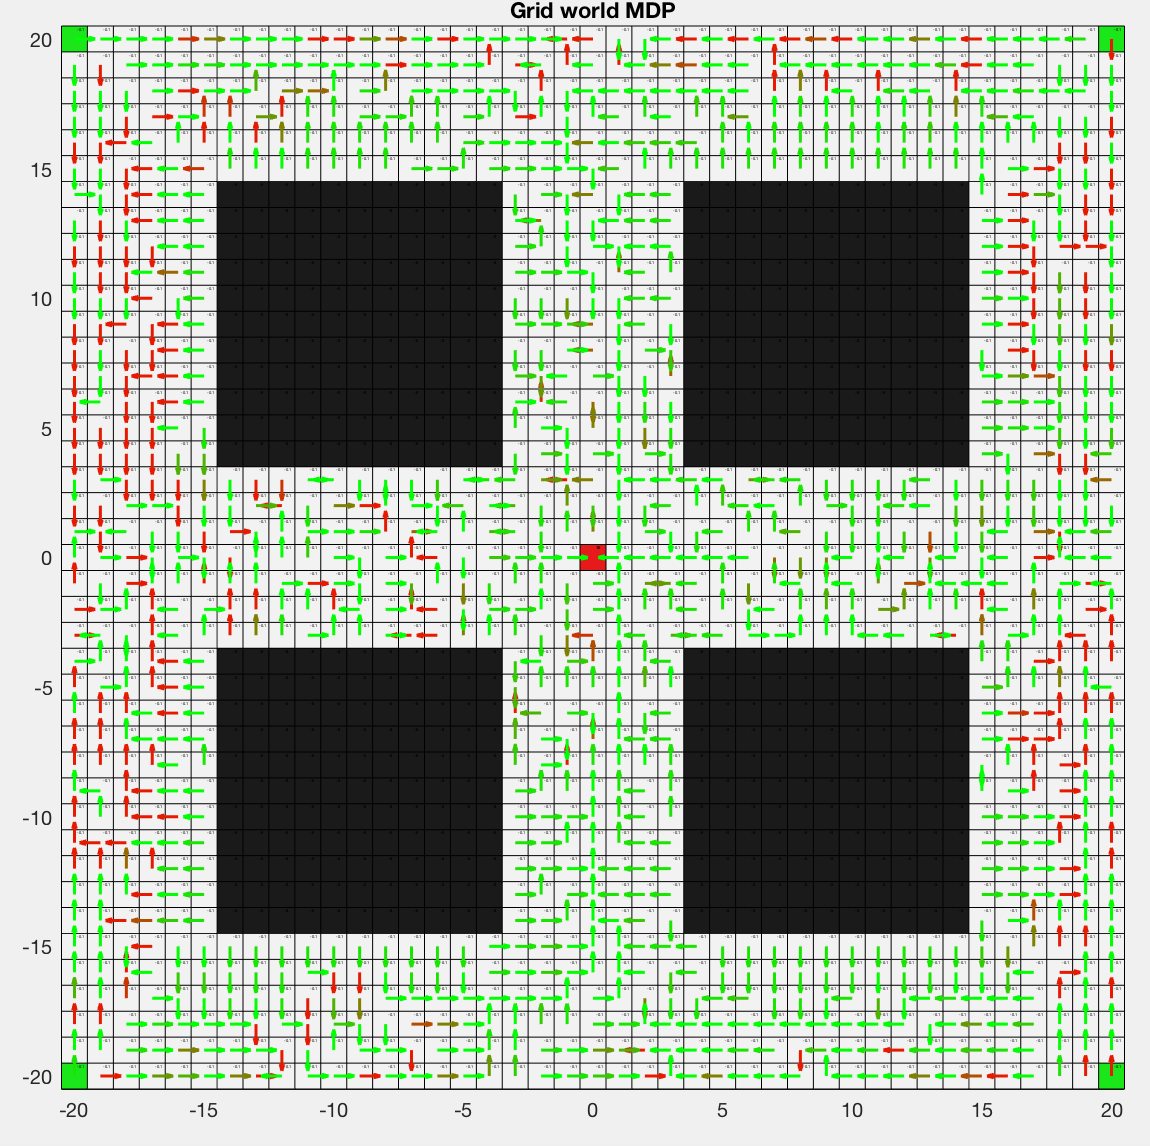
\includegraphics[width=0.95\linewidth]{heatmap_confidence_50}
							\caption{Learnt confidence : green arrows show near 1 posterior mean, red arrows near 0}
							\label{fig::heatmap_confidence_50}
						\end{center}
					\end{minipage}
				\end{figure}
				
				\paragraph{} The first observation one can make is that most of the suboptimal mentor actions are indeed well classified by the learner (red arrows). Also, most of the actions leading to such actions are also classified as poor recommandations, because they have a tendency of leading to deadlocks, or suboptimal actions.  
			}
		}
		\section{Explicit compliance}
		{
		
			\subsection{Practical considerations}
			{
				\paragraph{} The implementation of this method is rather straight forward and contains no major difficulties. However, some hyper-parameters have to be tuned, like the two temperatures (one for the initial MDP, the other for the above action selection) as well as their dynamics, and the update rule of (\ref{eq::av_update_rule}). 
				
				\paragraph{} In practice, this tuning is rather easy to perform, as long as one make sure that the initial values for $Q_c(s,l)$ and $Q_c(s,d)$ ($s\in\mathcal{S}$) don't absorb the observations but also retain some prior knowledge along the learning (the learning rate $\beta$ has to be related to those initial values in some way). 
			}
			\subsection{Results}
			{
				 \paragraph{} Figures (\ref{fig::av_il_subopt_120}) and (\ref{fig::av_il_subopt_50}) show the learning curves for an agent using the action-value compliant-based method, with two different suboptimal teachers. 
				 
				 \begin{figure}[ht!]
					\begin{minipage}{0.5\linewidth}
						\begin{center}
							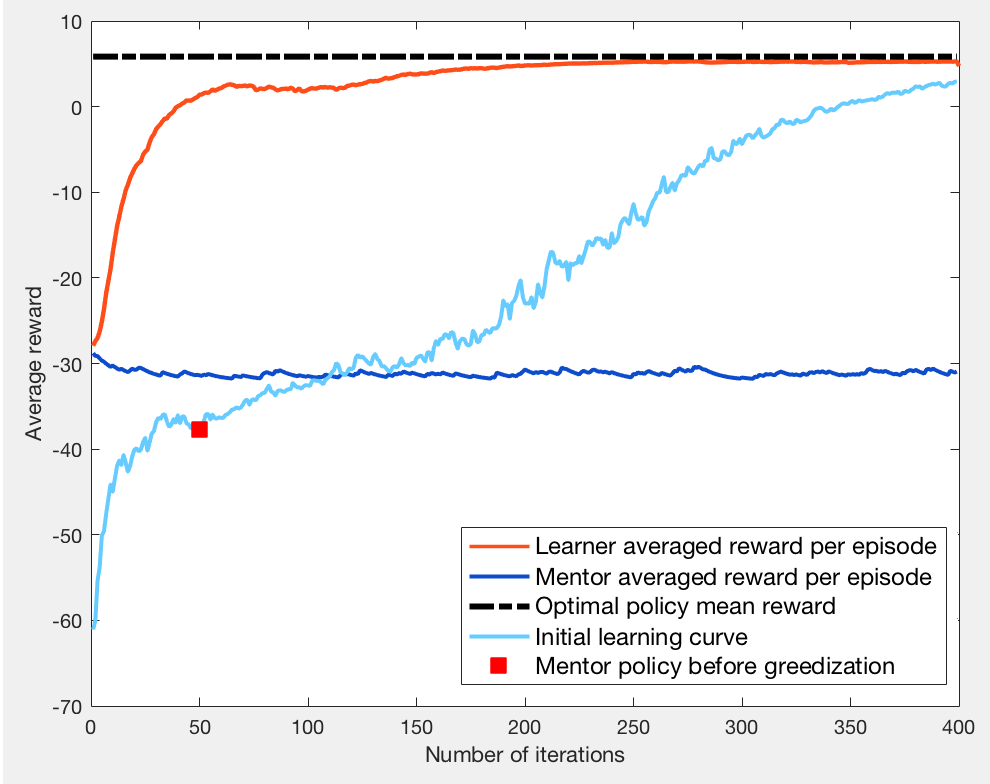
\includegraphics[width=0.95\linewidth]{av_il_subopt_120}
							\caption{Actor-critic learnt compliance learning curve for }
							\label{fig::av_il_subopt_120}
						\end{center}
					\end{minipage}
					\begin{minipage}{0.5\linewidth}
						\begin{center}
							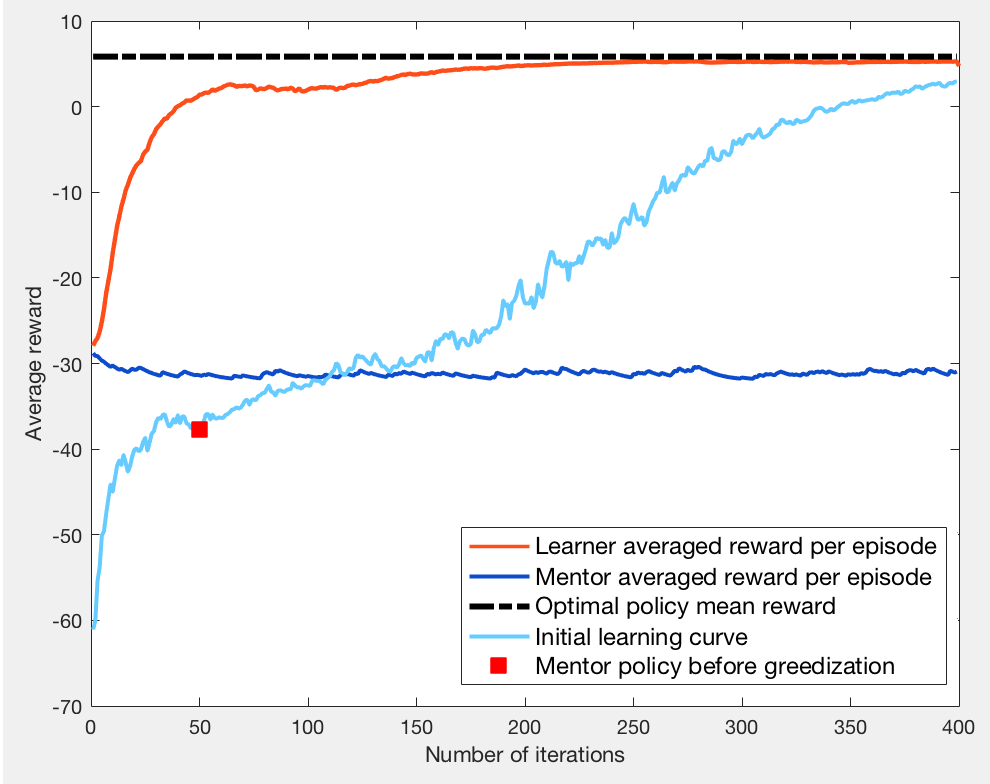
\includegraphics[width=0.95\linewidth]{av_il_subopt_50}
							\caption{Actor-critic learnt compliance learning curve}
							\label{fig::av_il_subopt_50}
						\end{center}
					\end{minipage}
				\end{figure}
				
				\paragraph{} As for the $\beta$-implicit method, we are able to reduce or even suppress the undershoot that the vanishing compliance method displayed, and to obtain fast convergence. 				
			}
			\subsection{Discussion}
			{
				\paragraph{} Similar plots of posterior result as for the actor-critic can now be drawn. Figures (\ref{fig::post_des_120}) and (\ref{fig::post_des_50}) display the histograms distributions for the action 'listen' and 'discard' (computed by the sigmoid value at end temperature). Figures (\ref{fig::heatmap_des_120}) and (\ref{fig::heatmap_des_50}) show the learnt decisions over the action-state space. 
				
				
				\begin{figure}[ht!]
					\begin{minipage}{0.5\linewidth}
						\begin{center}
							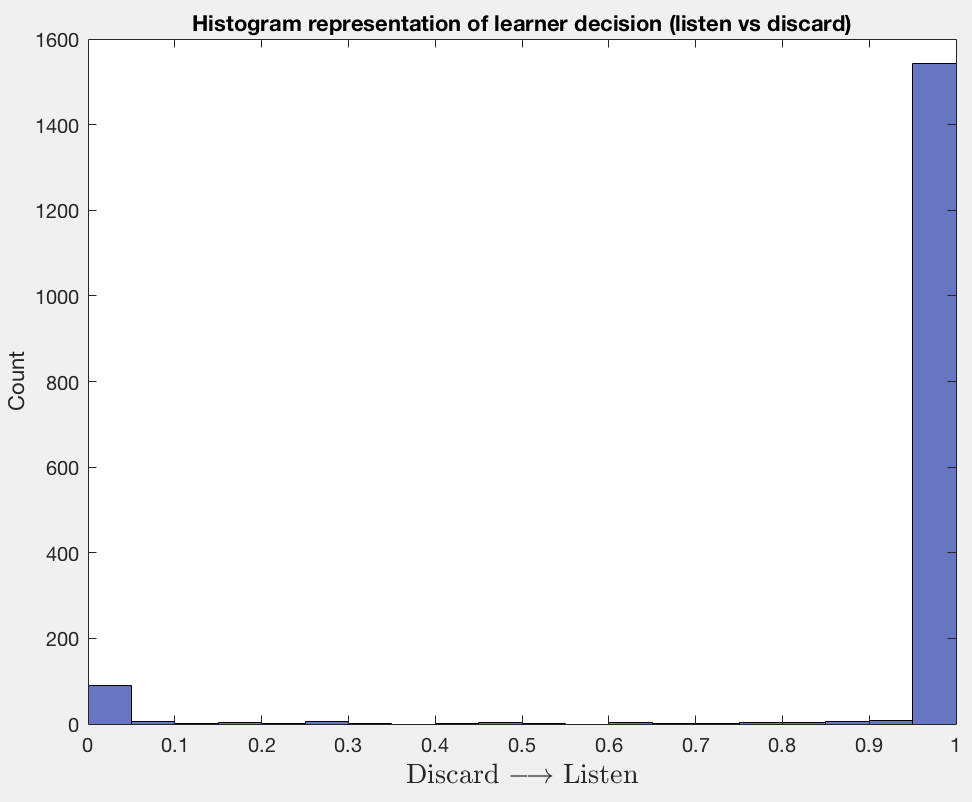
\includegraphics[width=0.95\linewidth]{pos_des_120}
							\caption{Histogram representation of the posterior decisions for a suboptimal teacher}
							\label{fig::post_des_120}
						\end{center}
					\end{minipage}
					\begin{minipage}{0.5\linewidth}
						\begin{center}
							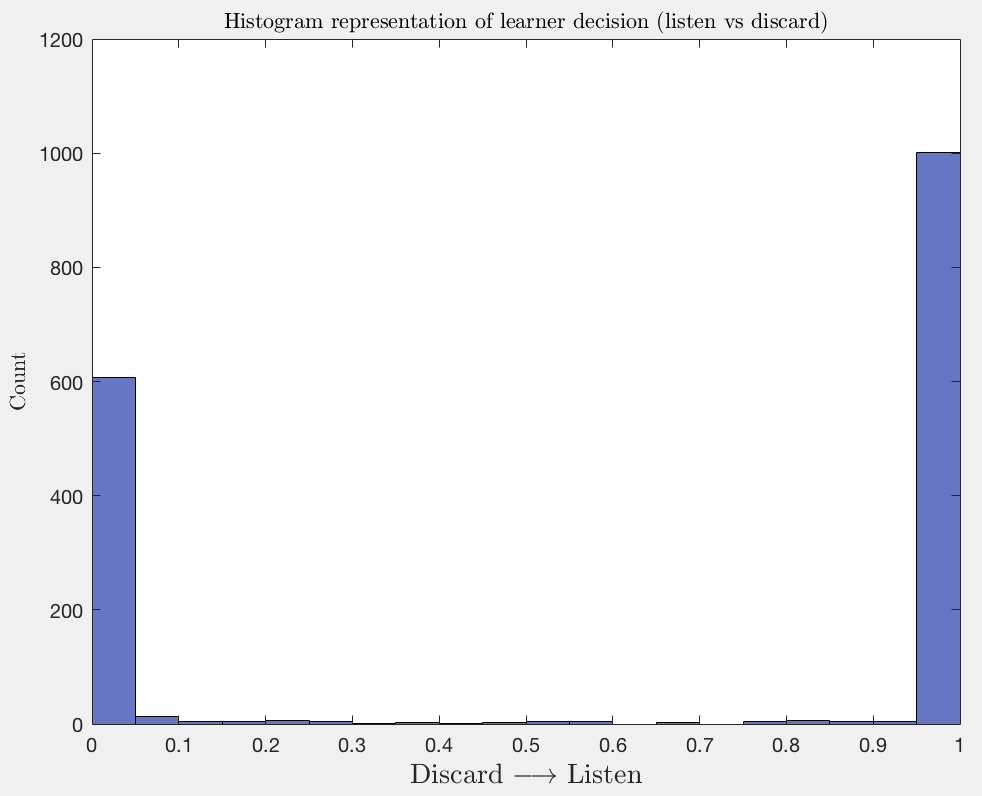
\includegraphics[width=0.95\linewidth]{pos_des_50}
							\caption{Histogram representation of the posterior decisions for a even more suboptimal teacher}
							\label{fig::post_des_50}
						\end{center}
					\end{minipage}
				\end{figure}
				
				
				\begin{figure}[ht!]
					\begin{minipage}{0.5\linewidth}
						\begin{center}
							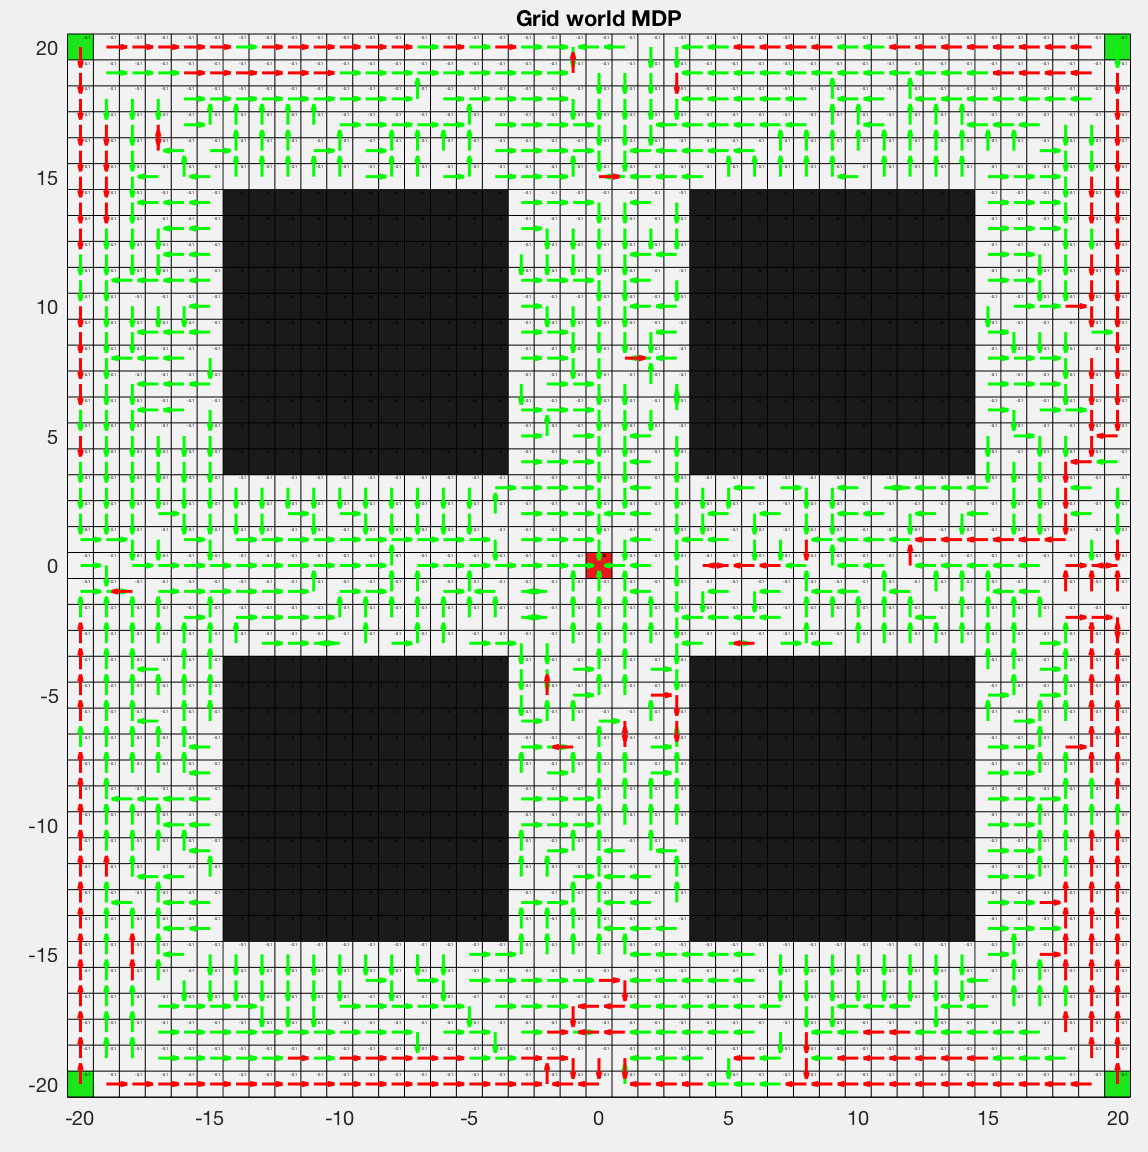
\includegraphics[width=0.9\linewidth]{heatmap_decision_120}
							\caption{Learnt decisions : green arrows show listening, red arrows discarding}
							\label{fig::heatmap_des_120}
						\end{center}
					\end{minipage}
					\begin{minipage}{0.5\linewidth}
						\begin{center}
							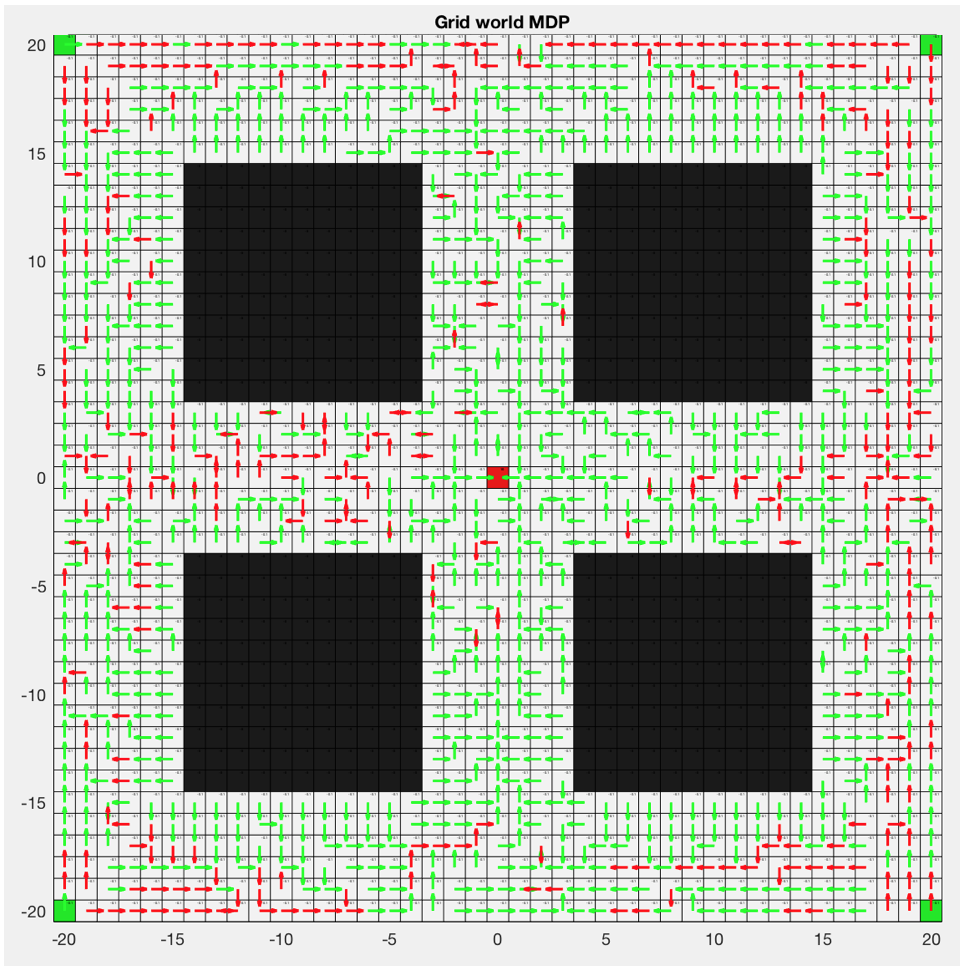
\includegraphics[width=0.9\linewidth]{heatmap_decision_50}
							\caption{Learnt decisions : green arrows show listening, red arrows discarding}
							\label{fig::heatmap_des_50}
						\end{center}
					\end{minipage}
				\end{figure}
			
			\paragraph{} Again, one can see that most wrong recommandations are well-classified. However, this method as a tendency to classify an action leading to a suboptimal sequence (in the mentor's policy) as a poor action. This as for consequence that the learner will try to always to go round the mentor's suboptimal recommandation, and sometime by making some detours. 
			}
		}
		\section{Algorithms comparaison}
		{
			\label{sec_method_comp}
			\paragraph{} We hereinafter focus on comparing the last three methods (vanishing compliance, implicit $\beta$-compliance and explicit compliance) between themselves and with classical reinforcement learning algorithms. 
			
			\subsection{Compliant learners}
			{
				\paragraph{} Let us now compare the different compliant learners between them. Figures (\ref{fig::compliant_comp_120}) and (\ref{fig::compliant_comp_50}) display the learning curves derived in the previous section altogether. If the $\beta$-implicit and the explicit compliance methods seem to behave better than the vanishing learner, it seems that the speed of convergence of all three algorithms tends to equalize as the teacher sub-optimality grows. This behavior is confirmed by figures (\ref{fig::metric_tt}) and (\ref{fig::metric_tr}). 
				
				\begin{figure}[ht!]
					\begin{minipage}{0.5\linewidth}
						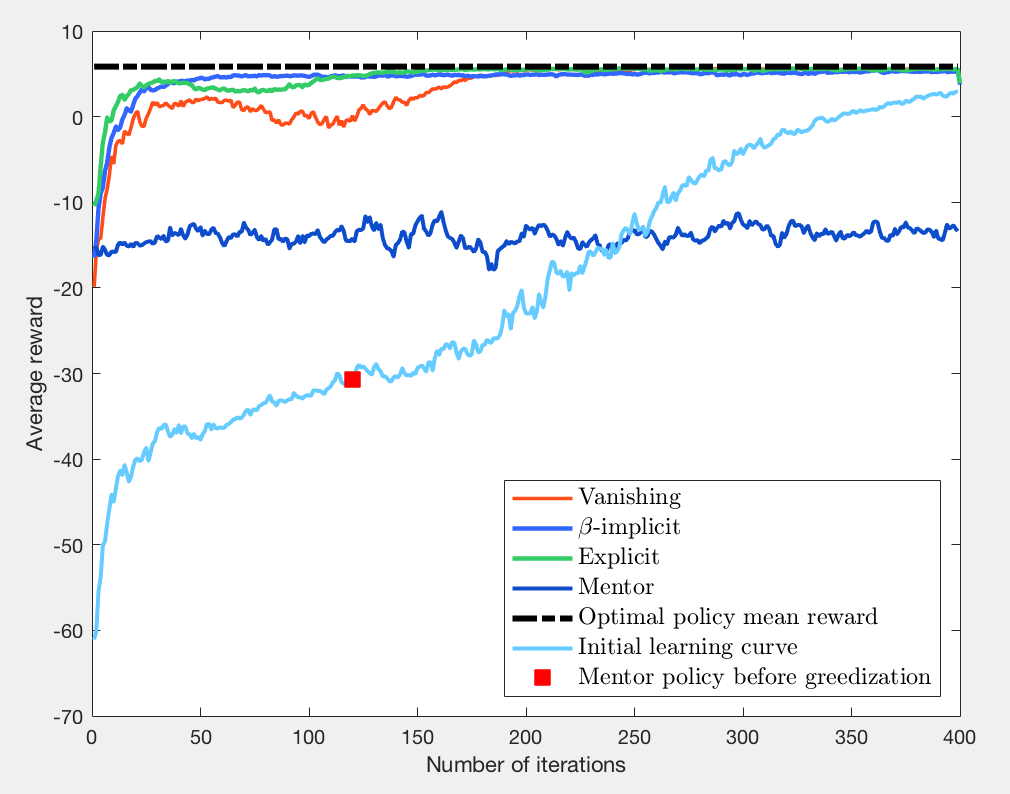
\includegraphics[width=\linewidth]{fullcomp_subopt_120}
						\caption{Learning curves for a first teacher}
						\label{fig::compliant_comp_120}
					\end{minipage}
					\begin{minipage}{0.5\linewidth}
						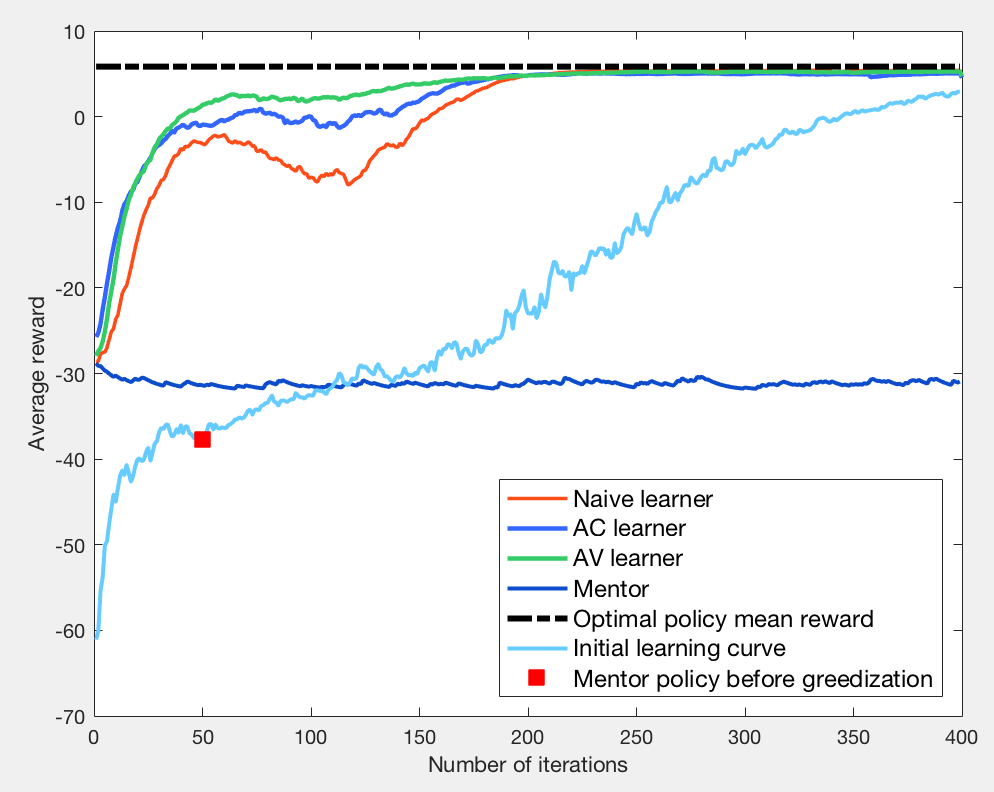
\includegraphics[width=\linewidth]{fullcomp_subopt_50}
						\caption{Learning curve for a second teacher}
						\label{fig::compliant_comp_50}
					\end{minipage}
				\end{figure}
				
				\paragraph{} In figures (\ref{fig::metric_tt}) and (\ref{fig::metric_tr}), different teachers are being tested based on their optimality level. This scalar measure of optimality is computed from a linear scaling between the random policy and the optimal policy mean expected return on one run. As one can see, the time to convergence for all methods seem to equalize as the optimality of the teacher decreases. However, the average accumulated reward until convergence is always better for the two adaptive methods - traducing the absence of the undershoot and better behaving methods. Hence, if our algorithms can't always speed up the learning (compared to a naive compliant learner), they \emph{provide better behaving agents}. 
				
				\begin{figure}[ht!]
					\begin{minipage}{0.5\linewidth}
						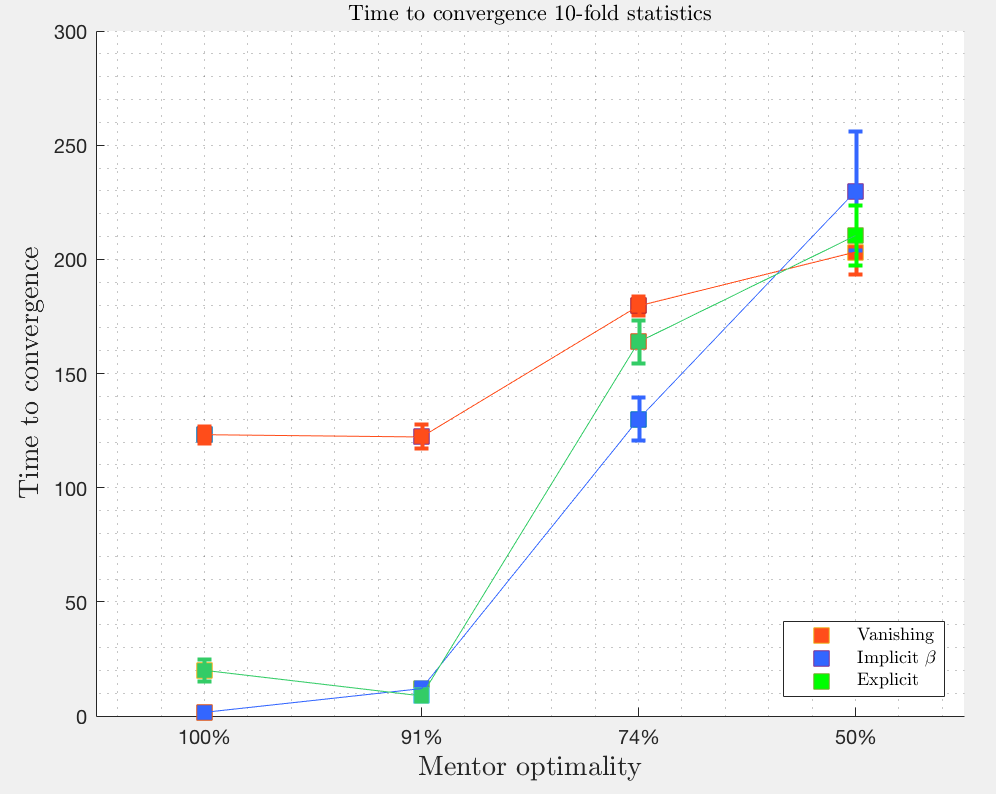
\includegraphics[width=\linewidth]{tt_metric}
						\caption{Time to convergence metric}
						\label{fig::metric_tt}
					\end{minipage}
					\begin{minipage}{0.5\linewidth}
						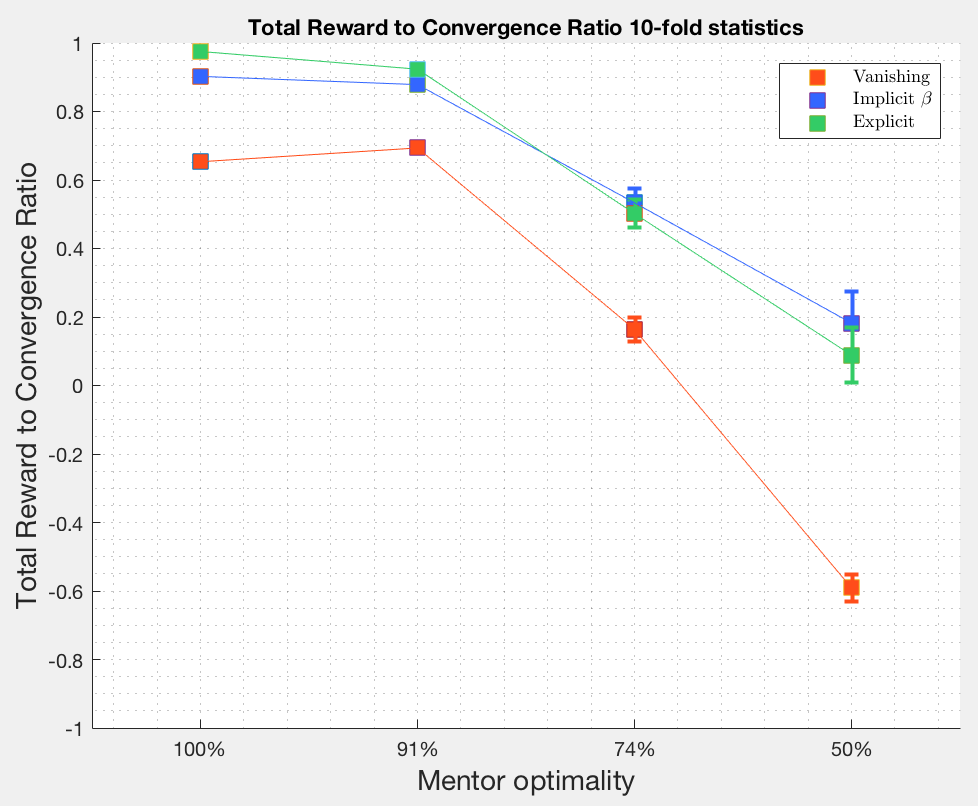
\includegraphics[width=\linewidth]{tr_metric}
						\caption{Reward to convergence metric}
						\label{fig::metric_tr}
					\end{minipage}
				\end{figure}	
			}
		}
		\subsection{Classical learners}
		{
			\paragraph{} As reminded in the beginning of this document, one of the goals of learning to demonstration is to speed up the learning. The goal of this section is to compare the behavior of the compliant-based learners we developed with some more classical reinforcement learning. 
			
			\paragraph{} Figures (\ref{fig::loner_comp_50}) and (\ref{fig::loner_comp_120}) display the learning curves of the compliant learner opposed with, respectively, TD(0) learners and TD($\lambda$) learners. As one can see, our algorithms performs way better than TD(0) learners, even with largely suboptimal teachers. However, they performed as well or even slightly worse than TD($\lambda$) learners. This phenomenon is mostly due to the fact the behind its action selection, our learners update their Q-values thanks to SARSA updates (on-policy). Generalizing to an off-policy update, and eventually by making use of eligibility traces will most likely improve the learning speed and beat TD($\lambda$) learners. 
							
				\begin{figure}[ht!]
					\begin{minipage}{0.5\linewidth}
						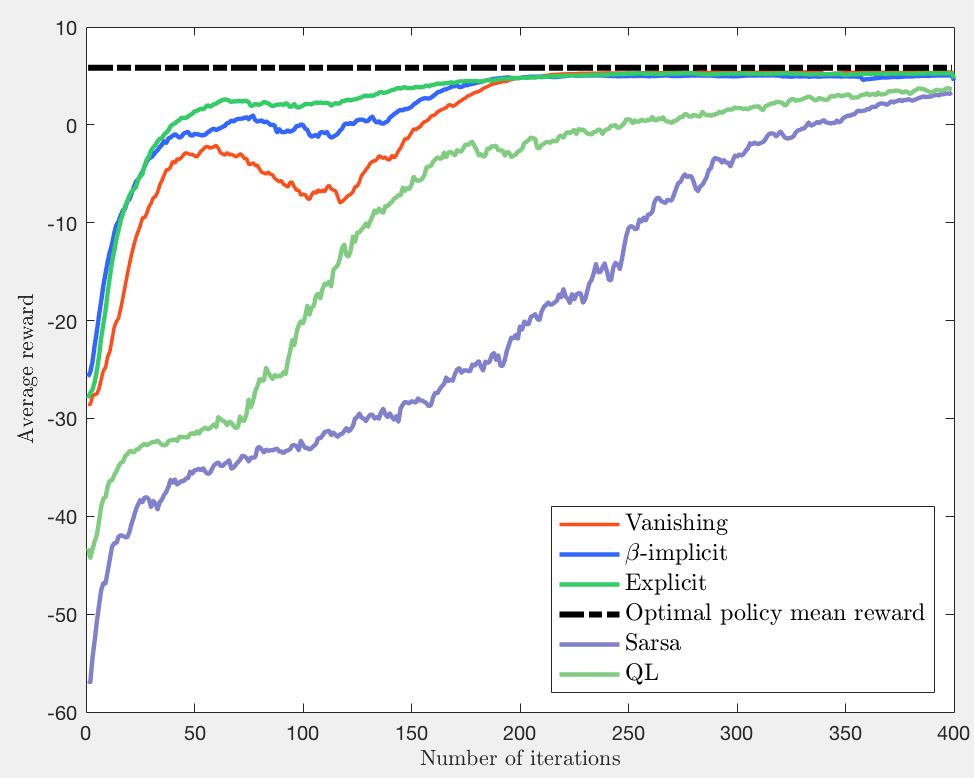
\includegraphics[width=\linewidth]{loner_comp_50}
						\caption{Method comparaison (teacher optimality : 50\%)}
						\label{fig::loner_comp_50}
					\end{minipage}
					\begin{minipage}{0.5\linewidth}
						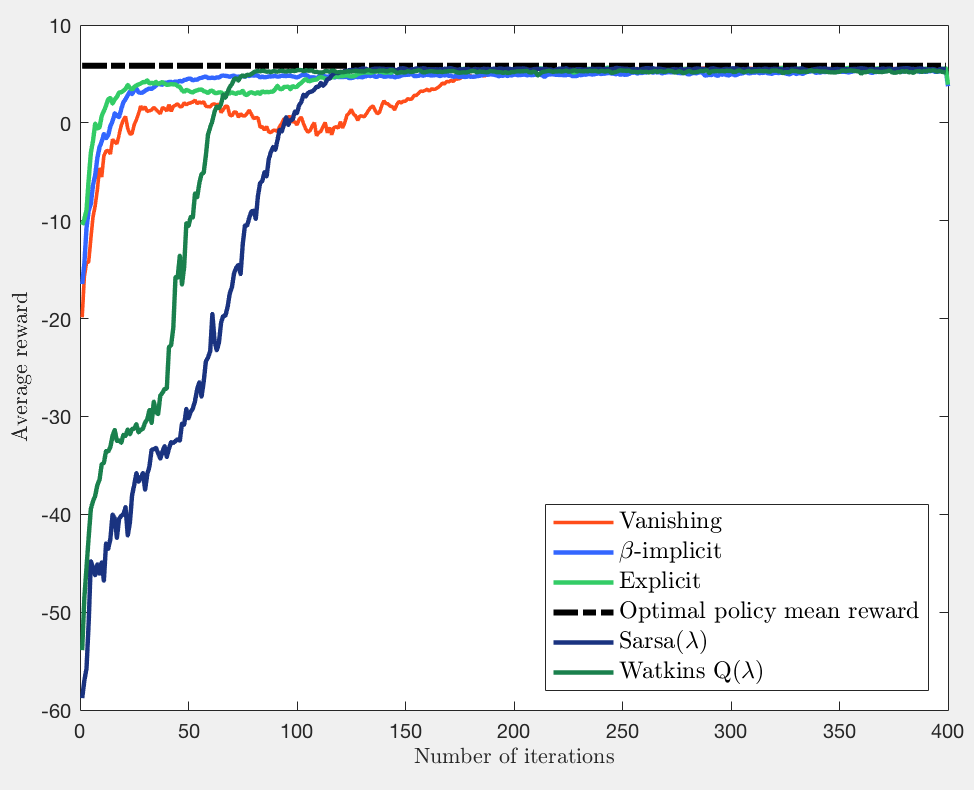
\includegraphics[width=\linewidth]{loner_comp_120}
						\caption{Method comparaison (teacher optimality : 75\%)}
						\label{fig::loner_comp_120}
					\end{minipage}
				\end{figure}
		}
	}
	
	\section{Improvements}
	{
		% Off-policy learning from the teacher 
	}
	\chapter*{Conclusion}
	\addcontentsline{toc}{chapter}{Conclusion}
	{
		\section{Outline}
		{

		}
		\section{Applicability}
		{
		
		}
		\section{Possible improvements}
		{

		}
	}
	
	
	
	\bibliographystyle{alpha}
 	 \bibliography{bibfile}
	 \nocite{*}
  
\end{document}